\chapter{Frontend Explained}

In this chapter I will document the contents of the frontend project and challenges met along the development process.

\section{Project Configuration}
\subsection{NextJS}

\noindent As discussed in the \textbf{Architecture and Choice of Technology} chapter, the frontend is built with NextJS 14. The project is configured to use TypeScript, Tailwind, ESLint, and the App Router.
\\\\
\noindent The App Router defines rules for creating routes within the application. For more details, see the project structure of an App Router application here \cite{nextjs-app-router-folders}. Although components can be placed directly in the App Router, only routes are placed inside it to maintain separation of concerns. While it was not possible to have separate app folders for each module, a minimum distinction is created by having different folders for each module inside the app folder, such as \textbf{main}, \textbf{(courses)}, and \textbf{(users)}. Folders with names in round brackets are interpreted as not being part of the route, thus providing only grouping capabilities.
\\\\
\noindent Throughout the application, environment variables are used to specify settings such as OAuth2 client secrets and other configuration variables needed throughout the application. Notably, these include the URLs to the backend modules, which can be accessed both in development mode and in production. NextJS by default allows the existence of three files: \textbf{.env.development}, which is used only in development mode, \textbf{.env.production}, which is used only in production, and \textbf{.env*}, which can override any value provided in the previous two files. There are also two types of environment variables within those files: private ones that are not accessible on the client side, ensuring they don't accidentally leak, and publicly available ones that are also added on the client side. To recognize a variable as a publicly available one, it needs to start with the prefix \texttt{NEXT\_PUBLIC\_}. \textbf{Attention!} It is important to take into account that \texttt{NEXT\_PUBLIC\_} variables are hardcoded and replaced with their values at project build time. This makes them immutable, so they should be properly set before the build. More information regarding how environment variables are handled by NextJS can be found here \cite{nextjs-env-variables}.

\subsection{VSCode + Extensions}

\noindent The coding environment utilizes VSCode with several helpful extensions. Custom configurations are added in the \textbf{.vscode} folder, inside a \textbf{settings.json} file, to tailor the project setup. To enhance development efficiency, the following extensions are employed: One Dark Pro, ESLint, npm Intellisense, Path Intellisense, Tailwind CSS Intellisense, Auto Rename Tag, Babel JavaScript, JavaScript and TypeScript Nightly, and Prettier. These extensions facilitate development by providing an aesthetically pleasing editor, offering suggestions for autocomplete and refactoring, highlighting potential syntax or logic errors in the code, and formatting all frontend code according to a customized standard. 
\\\\
\noindent The content of the \texttt{settings.json} file is presented below. It contains editor settings as well as extension settings that override the default ones.
\\\\
 \noindent The setting \textbf{"editor.defaultFormatter": "esbenp.prettier-vscode"} specifies Prettier as the default formatter for the editor, ensuring consistent code formatting. The setting \textbf{"editor.formatOnSave": true} enables automatic formatting of the code each time a file is saved. Under \textbf{"editor.codeActionsOnSave"}, \textbf{"source.fixAll.eslint": "explicit"} and \textbf{"source.addMissingImports": "explicit"} ensure that ESLint fixes all fixable issues and adds any missing imports when the file is saved. The \textbf{"files.associations"} section associates \texttt{.css} files with the Tailwind CSS language mode for better syntax highlighting and IntelliSense support. Various Prettier settings are defined to standardize the code style: \textbf{"prettier.tabWidth": 2} sets the tab width to 2 spaces, \textbf{"prettier.useTabs": false} ensures spaces are used instead of tabs, \textbf{"prettier.semi": true} enforces the use of semicolons, \textbf{"prettier.singleQuote": false} and \textbf{"prettier.jsxSingleQuote": false} enforce the use of double quotes for JavaScript and JSX respectively, \textbf{"prettier.trailing-\\Comma": "es5"} requires trailing commas where valid in ES5 (such as objects, arrays, etc.), and \textbf{"prettier.arrowParens": "always"} ensures parentheses are always used around arrow function parameters. For TypeScript React files, the default formatter is again set to Prettier with \textbf{"typescriptreact" : { "editor.defaultFormatter": "esbenp.prettier-vscode" }}.

\subsection{Tailwind}

\noindent Tailwind CSS is automatically integrated by NextJS, but further customization is done via \textbf{tailwind.config.ts}. Besides the configuration, custom styles are defined inside the \hl{/styles} folder. The main CSS file is \textbf{globals.css}, in which the other CSS files are imported. The \textbf{globals.css} file is then imported in the root layout of the frontend application. For this web platform, CSS files are mainly used to declare variables and add custom classes in one of the three layers of Tailwind: \textbf{base}, \textbf{components}, and \textbf{utilities}. The \textbf{base} layer is used for applying global styles and setting up foundational styles such as resets and typographic defaults. The \textbf{components} layer is for defining custom component styles, such as buttons and cards, ensuring consistency across the application. The \textbf{utilities} layer consists of utility classes that can be applied directly in the HTML to modify individual elements, providing a high degree of flexibility and control over styling. 
\\\\
\noindent The \textbf{tailwind.config.ts} file provides an easy way to extend the default theme and override or create new CSS classes. Besides extending the theme, the config file is used to specify the files that use Tailwind. The config file also allows the extension of Tailwind CSS with plugins, such as \textbf{tailwindcss-animate} and \textbf{@tailwindcss/container-queries}. These plugins enhance the functionality of Tailwind by adding additional utilities and features, making it more versatile and powerful for complex styling needs.

\subsection{Middleware}

\noindent In previous versions, I have referred to the backend created by NextJS as the middleware of the application. In this subsection, I am referring to the middleware configuration within NextJS, specifically the interceptor of requests between the client and the backend of NextJS. The middleware of this NextJS project is handled via the \textbf{middleware.ts} file. This file exports two main objects: a \textbf{NextMiddleware} function that receives a request and returns a NextResponse, and a \textbf{config} object which provides extra settings for the middleware. For example, the \textbf{config} object can define a pattern for matching routes, ensuring that not all routes will be affected by the NextMiddleware function. More information regarding the logic inside the auth middleware can be found in the security section.

\section{Folder structure}

In Figure \ref{fig:figure5}, the folder structure of the frontend project is presented. It is noticeable at first sight that some folders repeat themselves, appearing both at the root of the project and inside a module. This is intentional, as the folders have the same purpose wherever they appear. The difference between them is that the root folders are more general, meaning they can be used across all modules, while the nested folders are specific to the module they belong to.

\begin{figure}[h]
    \centering
    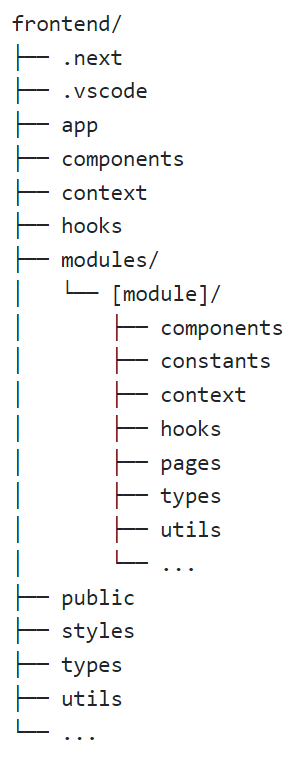
\includegraphics[scale=0.75]{images/frontend-folder-structure.png}
    \caption{Frontend - Folder structure}
    \label{fig:figure5}
\end{figure}

\noindent The \textbf{.next} folder contains bundled files essential for development mode, including cache of fetch requests and other metadata required for the NextJS project to function. Occasionally, I encountered random errors with the bundler, which were resolved by deleting this folder along with the \textbf{node\_modules} folder and allowing them to regenerate.
\\\\
\noindent The \textbf{.vscode} folder, previously discussed, contains the \textbf{settings.json} file, which specifies the extension properties to override in VSCode. This folder becomes completely unnecessary if a different text editor is used.
\\\\
\noindent The \textbf{app} folder is designated for NextJS's App Router and contains the folder tree that maps to various routes within the frontend application.
\\\\
\noindent The \textbf{components} folder contains reusable UI components that are used throughout the application. Components are the building blocks of the user interface, encapsulating markup, styles, and behavior. By organizing them in a dedicated folder, you ensure that they are easily accessible and can be reused across different parts of the application. This promotes consistency and reduces duplication. 
\\\\
\noindent The \textbf{hooks} folder contains custom React hooks. Hooks are functions that allow you to use state and other React features without writing a class. Custom hooks enable the reuse of stateful logic between components. By placing these hooks in a dedicated folder, the shared logic such as data fetching, form handling, or authentication is modularized and can be used across multiple components.
\\\\
\noindent The \textbf{context} folder is used for React Context API files. Context provides a way to pass data through the component tree without having to pass props down manually at every level. By using a context folder, global state or configuration that needs to be accessible throughout the application, such as theme settings or user authentication status, are managed and organized. This ensures that the context definitions and providers are centrally located and easy to manage.
\\\\
\noindent The \textbf{constants} folder contains constant values used across the application. By centralizing these values, the application ensures that they are defined in one place, making them easy to update and reducing the risk of hardcoded values scattered throughout the codebase. This practice improves maintainability and clarity, as developers can quickly locate and modify constants as needed.
\\\\
\noindent The \textbf{types} folder is dedicated to TypeScript type definitions. Type definitions help ensure that the code is type-safe, providing better tooling support, such as autocompletion and error checking. By placing important and reusable type definitions in a single folder, the NextJS project maintains a clear structure and make it easy to manage and reference types across the application. This is especially useful in large codebases where consistent use of types can prevent bugs and improve code quality.
\\\\
\noindent The \textbf{utils} folder contains utility functions and helper methods that are used across the application. These functions perform common tasks that are not specific to any single component or module, such as formatting dates, manipulating arrays, or making API requests. By organizing these utilities in a dedicated folder, it promotes code reuse and keep the codebase DRY (Don't Repeat Yourself). This also makes it easier to test and maintain these utility functions independently of the components that use them.
\\\\
\noindent The \textbf{modules} folder simulates a multi-module architecture, with each child folder representing a module that defines its own structure. Each module typically contains folders such as components, types, utils, constants, context, hooks, and pages. This design allows for modular development, where each module can independently specify its own folders or omit unnecessary ones. The \textbf{pages} folder, unique to each module and absent in the root structure, defines pages and layouts imported into the \textbf{app} folder. This structure ensures that each module is self-contained and can manage its specific functionality while maintaining a coherent overall project organization.
\\\\
\noindent The folder structure presented in Figure \ref{fig:figure5} and previously explained was inspired by the project structure of other applications, but mostly by this blog post \cite{react-folder-structure}.
\\\\
\noindent When referencing files within this folder structure, it is important to use absolute paths instead of relative ones. Although this approach might break modularity, as moving a folder will invalidate the paths within it, it provides clarity regarding the overall location of the imported files. The @/ symbol is used to denote the root of the application, simplifying the process of locating and importing files across different modules. This practice ensures that file references are consistent and understandable, regardless of the specific module or directory from which they are being accessed.

\section{Themes and Design}

\subsection{Light and Dark}

\noindent The web platform offers two main themes: dark and light. Additionally, there is a "system" theme that selects between dark and light based on the preferences of the user's device.
\\\\
\noindent These themes are implemented using the \textbf{next-themes} package from npm. This package provides a \textbf{ThemeProvider}, which is placed in the root layout of the application. CSS variables for theme customization are declared at the \textbf{@base} Tailwind layer, within the \textbf{:root} and \textbf{.dark} modifiers. These variables dynamically switch between light and dark modes based on the selected theme.
\\\\
\noindent The package also offers a \textbf{useTheme} hook, which allows retrieval of the selected theme and the resolved theme. The selected theme can be light, dark or system, but the resolved theme will be either light or dark, depending on the device settings. The \textbf{useTheme} hook also provides a \textbf{setTheme} function to update the theme. Importantly, the package ensures that if dark mode is enabled, the light theme will not flicker before the dark theme loads, providing a smooth user experience.
\\\\
\noindent To apply custom styles on components with Tailwind CSS now becomes very simple. All classes that are prefixed by \textbf{dark:} will be applied only on dark mode.
\newpage
\begin{figure}[h]
    \centering
    \begin{minipage}{0.45\textwidth}
        \centering
        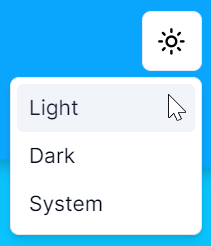
\includegraphics[width=0.5\linewidth]{images/theme-button-light.png}
        \caption{Theme Button - Light}
        \label{fig:theme-button-light}
    \end{minipage}%
    \hspace{0.1\textwidth}% 
    \begin{minipage}{0.45\textwidth}
        \centering
        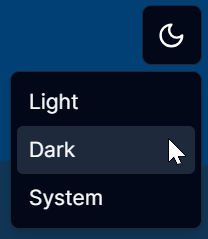
\includegraphics[width=0.5\linewidth]{images/theme-button-dark.png}
        \caption{Theme Button - Dark}
        \label{fig:ftheme-button-dark}
    \end{minipage}
\end{figure}

\noindent The user can easily change between themes using the button available on all pages, as shown in Figures \ref{fig:theme-button-light} and \ref{fig:ftheme-button-dark}. The button is implemented as a toggle switch, and will also change appearance based on the selected theme.

\subsection{Shadcn/UI}

\noindent Shadcn/UI is an open-source repository that offers accessible and customizable components implemented with \textbf{Tailwind CSS} and \textbf{Radix/UI Primitives}. Radix Primitives is a low-level UI component library focused on accessibility, customization, and developer experience. Shadcn \textbf{is not} a components library in the traditional sense, as components are not directly imported from a package. Instead, to use them, they need to be copy-pasted into the application, making the components as customizable as possible.
\\\\
\noindent The components taken from Shadcn \cite{shadcn-components} are placed in the \textbf{ui} folder within the root \textbf{components} directory. Although these components are fully editable, most are retained in their original source code with only minor modifications related to typography or the addition of extra variants. This approach ensures the components remain customizable while still adhering to the design standards of the application.
\\\\
\noindent The components provided by Shadcn integrate well with Next-Themes as well, having both light and dark modes.
\\\\
\noindent For installation, although the components can be manually copied, an automated option exists as well. Before using it, the \hl{npx shadcn-ui@latest init} command must be executed. This command configures download preferences for Shadcn, such as the components folder, TypeScript or JavaScript, CSS variables, component styles, and more. It also adds a utility function for merging multiple strings of classes, utilizing the \textbf{tailwind-merge} package, which is required within the source code of the components. After this initial setup, components can be downloaded via \hl{npx shadcn-ui@latest add <component>}.

\subsection{Typography}

\noindent Typography is an important aspect of the application, providing a subconscious user experience based on how it is chosen. The first step in defining typography was deciding on a typography scale. There are three main categories of typography scales: high contrast, medium contrast, and low contrast.
\\\\
\textbf{High Contrast:} This scale features significant size differences between text elements, making it ideal for drawing attention to headings and titles. It's useful for creating a dramatic and impactful design.
\\\\
\textbf{Medium Contrast:} With a balanced difference in text sizes, this scale is versatile and suitable for a harmonious and readable design. It works well for body text, subheadings, and captions, providing clear hierarchy without being overwhelming.
\\\\
\textbf{Low Contrast:} Featuring subtle size differences, this scale creates a uniform appearance and is perfect for minimalist designs. It enhances readability and user comfort, making it ideal for content-heavy applications like articles and reports.

\begin{figure}[h]
    \centering
    \begin{minipage}{0.45\textwidth}
        \centering
        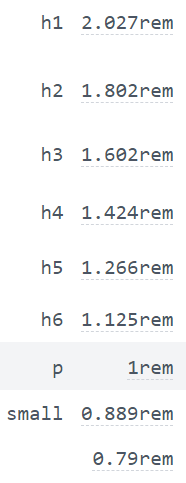
\includegraphics[width=0.5\linewidth]{images/typography-major-second.png}
        \caption{Major Second - 1.125}
        \label{fig:figure6}
    \end{minipage}%
    \hspace{0.1\textwidth}% 
    \begin{minipage}{0.45\textwidth}
        \centering
        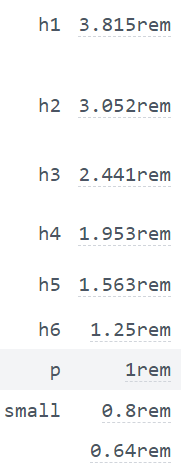
\includegraphics[width=0.5\linewidth]{images/typography-major-third.png}
        \caption{Major Third - 1.250}
        \label{fig:figure7}
    \end{minipage}
\end{figure}

\noindent For window sizes below \textbf{768px}, a major second typescale is applied, as depicted in Figure \ref{fig:figure6}. Conversely, for larger sizes, a major third typescale is utilized, as demonstrated in Figure \ref{fig:figure7}. Both fall within the \textbf{medium contrast} category, establishing a clear hierarchy while ensuring user engagement. % This approach facilitates distinct section separation while accommodating occasional heavier content.
\\\\
\noindent The typography scales mentioned above are implemented via custom Tailwind CSS classes (h1-typography, h2-typography, ..., p-typography, small-typography, caption-typography), which are directly applied to components. Occasionally, text size adjustments are made using Tailwind's text-[size] utility classes to improve page layout, but the overall design adheres to the specified scales.
\\\\
\noindent Adhering to NextJS's default settings, the web application adopts the \textbf{Inter} font. Alongside typography scale and font style considerations, factors such as letter and line spacing, color, and text decorators must be taken into account. Due to time constraints, emphasis has been placed on typography scale and font style, with other aspects being improvised to maintain an aesthetically pleasing design.

\subsection{Responsive}

\noindent Responsiveness is crucial for all web applications. Ensuring that a website looks good and works well on different devices and screen sizes is essential. Two strategies are employed inside the frontend application.
\\\\
\noindent Firstly, the web platform relies on Tailwind's responsive features, such as breakpoints for window sizes that conditionally activate classes when the minimum size is reached. Tailwind follows a mobile-first design approach, where styles are overridden from the smallest to the largest screen size.
\\\\
\noindent Secondly, a higher-order component is utilized to conditionally render content based on media queries. The \textbf{ConditionalRenderMediaQuery} component accepts three main parameters: \textbf{mediaQuery} (a string), \textbf{trueComponent} (a ReactNode), and \textbf{falseComponent} (a ReactNode). It can also receive additional parameters for server-side rendering configuration. This component leverages the \textbf{useMediaQuery} hook from the \texttt{usehooks-ts} library \cite{usehooks-ts}, which returns either true or false based on a media query string. Despite being marked as a client-side component, it can accept server-side components as parameters without converting them to client-side components. This is made possible by the inner workings of NextJS, which reserves slots for component parameters and renders the client-side component independently of the components received as parameters.
\\\\
\noindent An example of responsiveness can be seen in figures \ref{fig:main-page-desktop} and \ref{fig:main-page-mobile}, which display the different layout designs for desktop and mobile devices.

\section{Main Page}

The main page is designed to be minimalistic yet welcoming, with an attractive design and useful information. It focuses on transmitting three crucial pieces of information to the user:
\\\\
\noindent \textbf{Who are you?} This is conveyed through the web platform's logo and name, displayed in the navbar as DesignOOP. The name is suggestive and easy to remember, especially for courses related to object-oriented programming design patterns. The logo, generated with AI using \textbf{Bing AI}, represents building blocks surrounded by paintbrushes, signifying design.
\\\\
\noindent \textbf{What do you do?} This information is communicated through the suggestions card, which includes links to the community for user interaction, the official courses page, and the educational resources editor.
\\\\
\noindent \textbf{How can you help me?} This question is addressed through bullet points text on the main page, highlighting key benefits. Additionally, the suggestions card provides further assistance by offering relevant links and resources.

\begin{figure}[h]
    \centering
    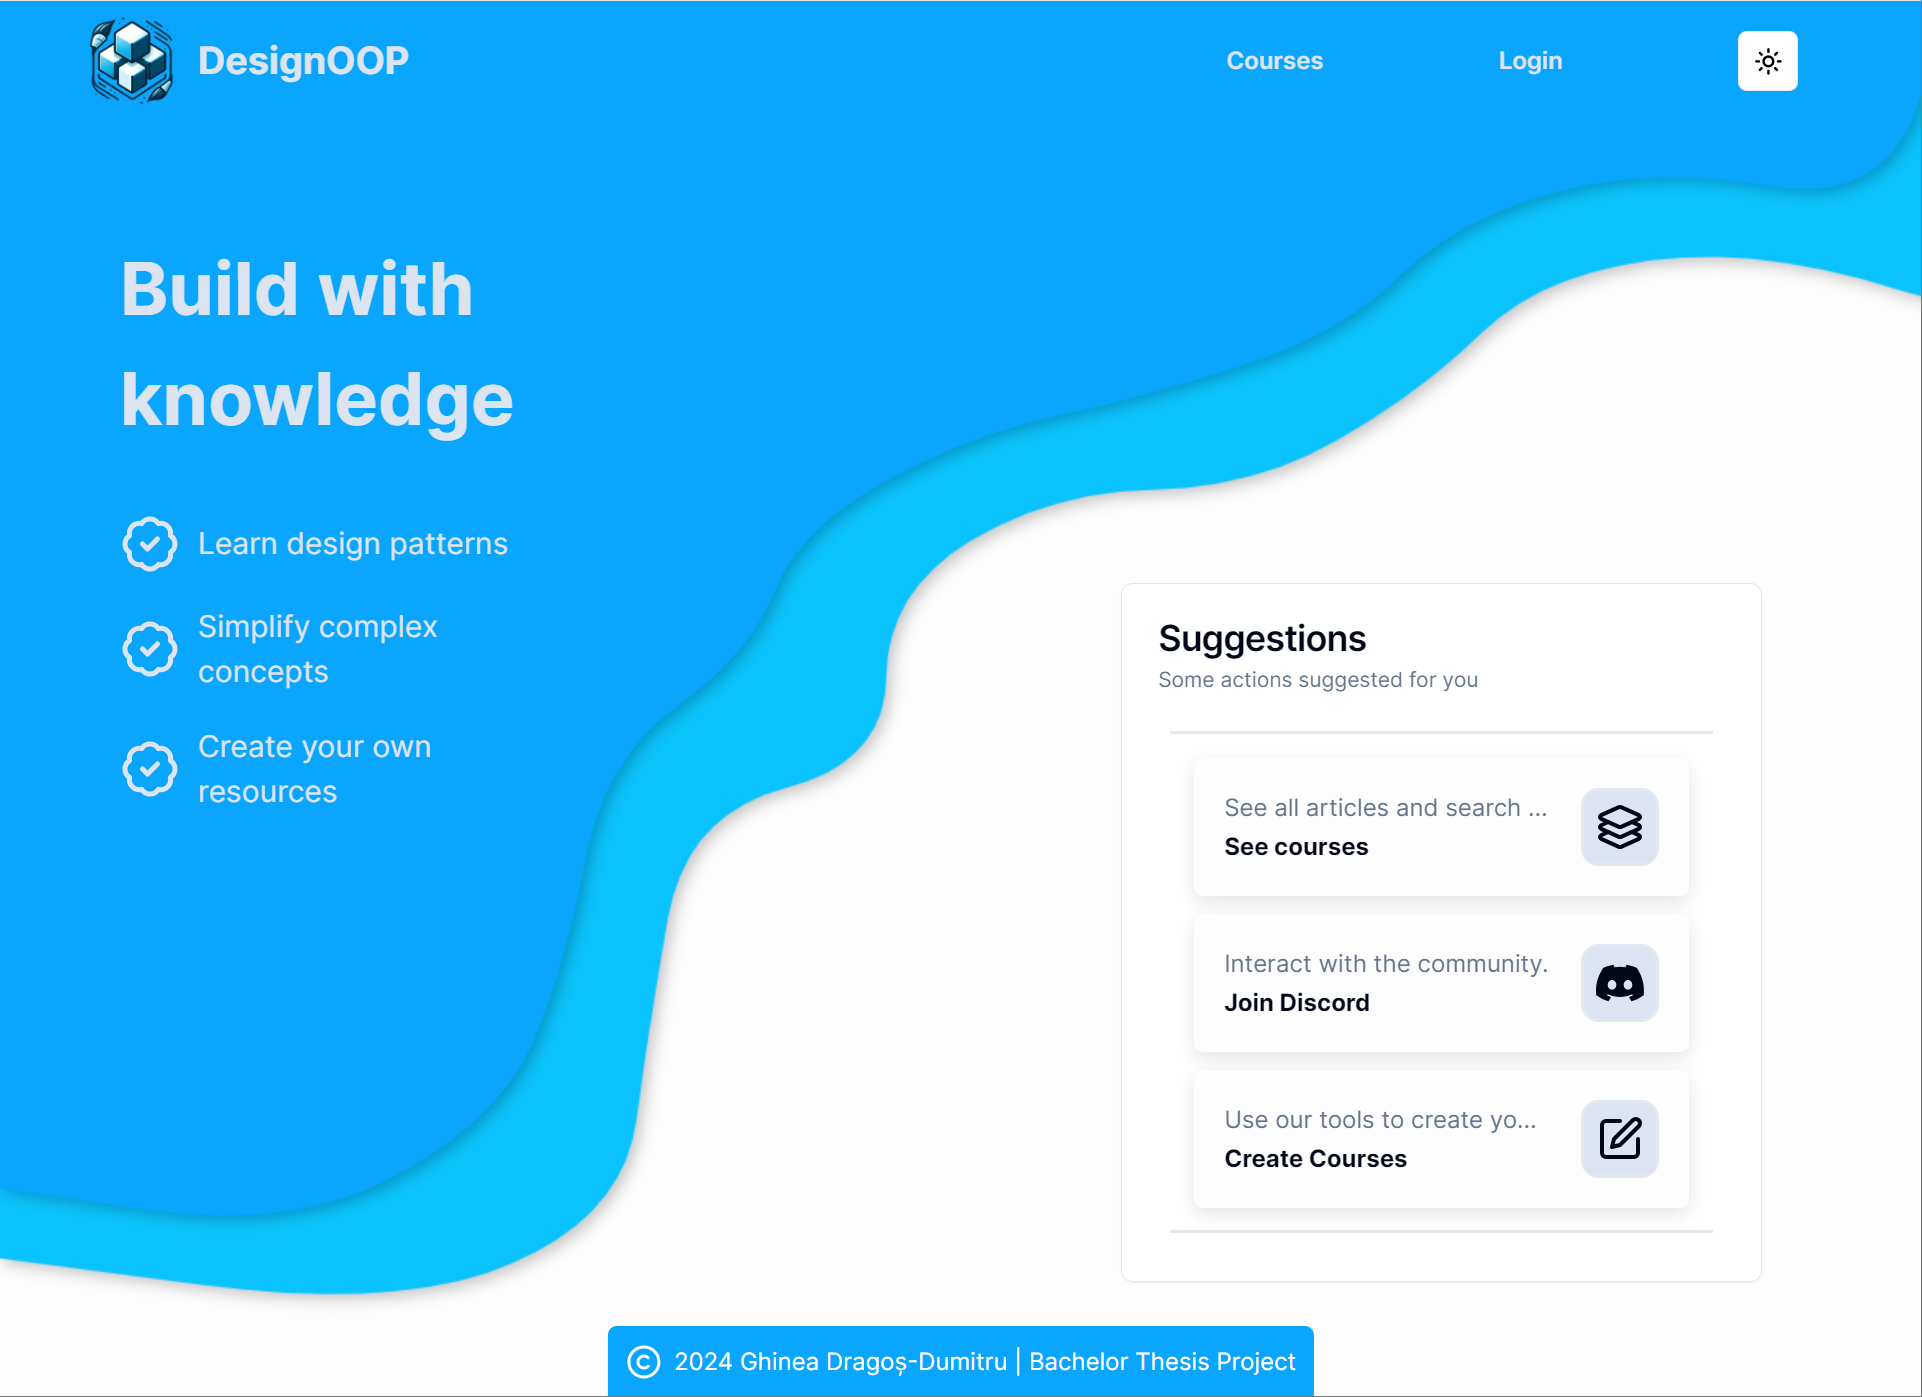
\includegraphics[scale=0.45, trim = {0 0 1 0}, clip]{images/main-page-desktop.png}
    \caption{Main Page - Desktop}
    \label{fig:main-page-desktop}
\end{figure}

\begin{figure}[h]
    \centering
    
\includegraphics[scale=0.4]{images/main-page-mobile.png}
    \caption{Main Page - Mobile}
    \label{fig:main-page-mobile}
\end{figure}

\subsection{Waves}

\noindent The wavy background with two layers is intended to create an organic, aesthetically pleasing look, providing a positive first impression of the application.
\\\\
\noindent When considering how to create the waves, \textbf{Bézier curves} were the first choice due to their ability to produce smooth and rounded lines. For the outline of the waves, cubic Bézier curves were utilized. Using an HTML canvas along with helper JavaScript functions to draw the curves and control points, a curve editor was created. This editor outputs the necessary control points to recreate the curve, with the coordinates normalized between 0 and 1, relative to the size of the canvas.
\\\\
\noindent The canvas shown in Figure \ref{fig:figure8} functions as a curve editor, allowing users to drag control points of multiple curves. The red dots indicate draggable control points, while the curves themselves are represented by green dots, placed closely together to form a continuous green line. In the canvas depicted, four Bézier curves are arranged next to each other, creating the appearance of a continuous wavy line. The canvas in Figure \ref{fig:figure8} has a square aspect ratio. For mobile waves, the same editing technique is employed, but instead of a square canvas, a slightly taller and narrower one is used. This adjustment ensures the waves are appropriately scaled and visually appealing on different screen sizes.

\begin{figure}[h]
    \centering
    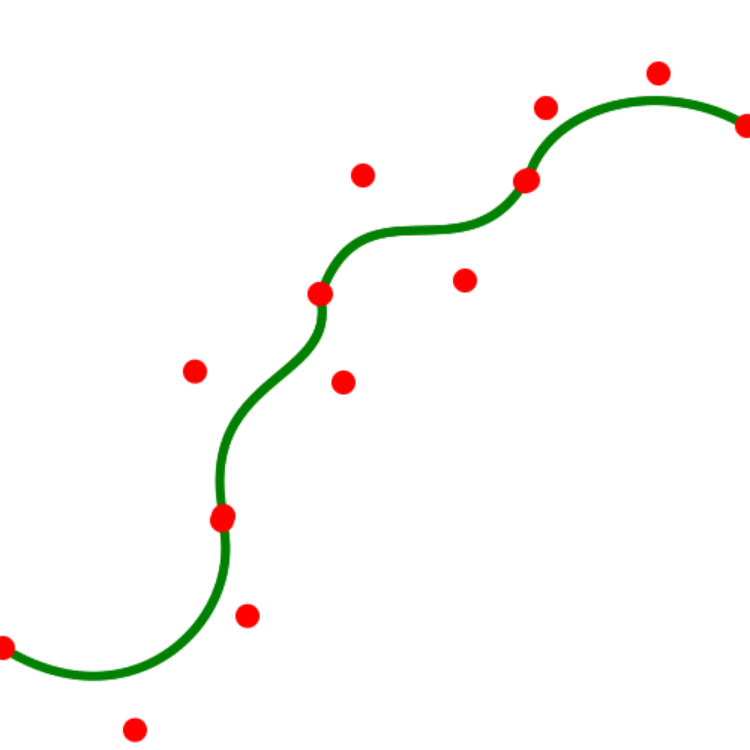
\includegraphics[scale=0.6]{images/bezier-curve-editor.png}
    \caption{Bézier curves in a canvas}
    \label{fig:figure8}
\end{figure}

\noindent After establishing the shape of the wave, the next step is to convert it into an actual surface. This is done by implementing the concept of \textbf{Bézier skin}. A Bézier skin is used on the main page to create a closed shape from Bézier curves based on control points. In Figure \ref{fig:figure9}, the control points are chosen as the top corners of the screen, to which the green dots are added. The green dots are generated along the curve established in Figure \ref{fig:figure8}. To make the wave move, the control points marked with green dots are moved diagonally back and forth, along a sinusoidal trajectory over time. For an organic feel, the dots are not moved back and forth simultaneously. To achieve a natural gradual randomization, \textbf{Perlin noise} is used.

\begin{figure}[h]
    \centering
    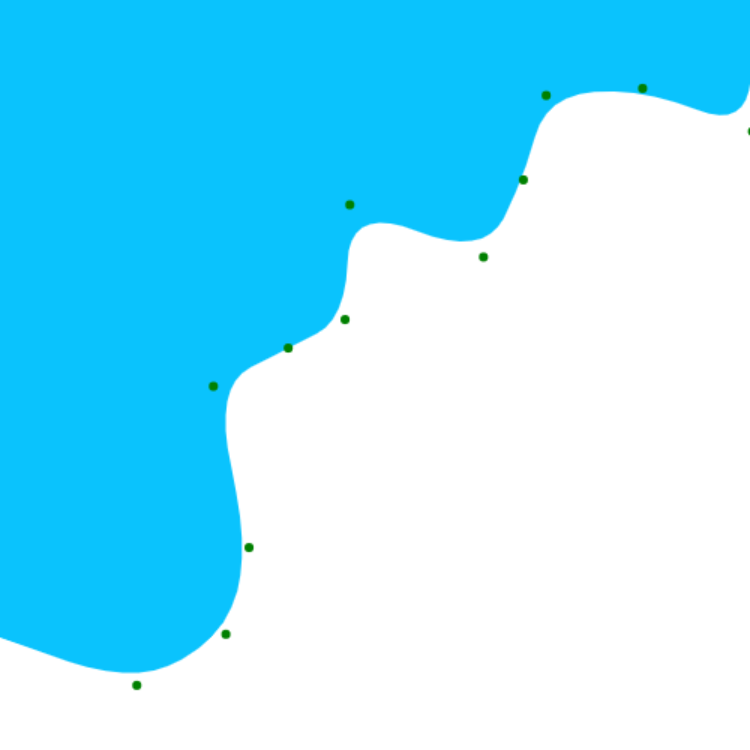
\includegraphics[scale=0.6]{images/bezier-wave-with-guides.png}
    \caption{Wave with guide points}
    \label{fig:figure9}
\end{figure}

\noindent After having the dynamic wave, the only thing left to obtain the final design is to add a shadow on it and combine it with another wave to offer depth perception. The final result is on the main page of the web platform.

\subsection{Navbar}

\noindent The navbar of the web platform contains multiple elements for quick access to other areas of the website. Firstly, there is the logo along with the web platform's name, which acts as a home button when clicked, loading the main page. Secondly, there is the courses button, which redirects to the courses section. Finally, there is the user profile button. If the user is not logged in, the button displays "Login"; for logged-in users, there are two buttons: one for accessing their profile and another for logging out.
\\\\
\noindent The navbar uses the \textbf{ConditionalRenderMediaQuery} higher-order component to selectively load a mobile navbar and a desktop navbar. The navbar component is not placed at the root level of the application but inside the layout of each module. Although the navbar might vary in design from section to section, it maintains a consistent look across all of them.
\\\\
\noindent To avoid the use of too many files, if the navbar requires a different style for a specific module of the application, a new variant is created, and Tailwind class names are added or removed accordingly. Currently, two variants exist: \textbf{main} (see Figure \ref{fig:navbar-main}) and \textbf{default} (see Figure \ref{fig:navbar-default}). If no variant is specified when the component is called, the default variant will be used.

\begin{figure}[h]
    \centering
    
\includegraphics[scale=0.55]{images/navbar-main.png}
    \caption{Navbar - Main Variant}
    \label{fig:navbar-main}
\end{figure}

\begin{figure}[h]
    \centering
    
\includegraphics[scale=0.55]{images/navbar-default.png}
    \caption{Navbar - Default Variant}
    \label{fig:navbar-default}
\end{figure}

\subsection{Suggestions}

\noindent The suggestions card currently directs users towards the three main uses of the application. Firstly, the \textbf{Join Discord} option connects users to a Discord community where they can interact with others who share an interest in design patterns and exchange knowledge. Secondly, the \textbf{See courses} option presents users with the official learning resources available on the web platform. Finally, the \textbf{Create courses} option redirects users to the educational resource creator, personalized in the style of the web application.
\\\\
\noindent A suggestion inside the suggestions box (Figure \ref{fig:suggestions-card}) consists of three components: a bolded title, a suggestive icon, and a description that is truncated but becomes fully visible on hover.

\begin{figure}[h]
    \centering
    
\includegraphics[scale=0.7]{images/suggestions-card.png}
    \caption{Suggestions box with hovered suggestion}
    \label{fig:suggestions-card}
\end{figure}

\noindent Although currently static, the suggestions could become more dynamic and user specialized in the future, by storing the user activity in their profile and recommend specific courses based on the visited ones.

\section{Profile}

The profile is part of the \textbf{users module}, along with the frontend security measures that will be covered in a later section.

\subsection{Details}

\noindent A user profile currently consists of their details (Figure \ref{fig:profile-card}). The profile page presents the avatar of the user along with their username, the linked providers, and the date they were connected. At the time of writing this thesis, there are two possible user providers: \textbf{Discord} and \textbf{GitHub}.
\\\\
\noindent Users are generated based on the emails from provider connections. If a user connects via GitHub, for example, with a specific email, and there is a user associated with that email, then the authentication request will resolve using that user. In case a user does not exist with that email, a new one is created and linked to the provider that resulted in the creation of the user. The initial profile picture along with the username are taken from the linked provider on user creation. If a linked provider changes their email, the linked provider's ID from the backend is automatically relocated to the new email.

\begin{figure}[h]
    \centering
    
\includegraphics[scale=0.7]{images/profile-card.png}
    \caption{Profile details card}
    \label{fig:profile-card}
\end{figure}

\subsection{Account Usage}

\noindent Currently, the accounts have only administrative purposes, being used for authorization. Authorization is required in the web application for course management. Although the course editor is open for everyone, even unauthenticated users, official courses can't be managed by anonymous people.
\\\\
\noindent In the future, accounts might serve an important role in managing data such as browsing history, which could facilitate a recommendation algorithm personalized to user preferences and needs. Besides that, a notifications center can be employed, providing users with direct messages if there are problems, opportunities to learn, or other things specific users might need to know. In the ecosystem of interacting with users, the possibilities are nearly endless.

\section{Courses}

The courses represent the main reason this web application exists. The frontend needs to provide valuable interfaces, both for reading the courses and creating them. To improve the user's experience multiple features are implemented, which are presented in the following subsections.

\subsection{Layout}

\noindent All pages from the courses module have a three-column layout, including as much information as possible in a structured way that is easily understood by people. On mobile, similar to this layout, only the middle section is displayed, but arrows on the sides of the screen allow the opening of the hidden sections as side sheets/dialogs. On top of this three-column layout is the global navbar of the application, refered to as the \textbf{static navbar}.
\\\\
\noindent The \textbf{left side} is a separate vertical navbar with specific options for the courses module. From this navbar, you can change between searching for courses, viewing your browsing history, and opening the course editor. The left side is meant to be somewhat generic for all pages from the module, but due to possible future extensions, the internal structure allows overwriting this navigation bar in any courses route.
\\\\
\noindent The \textbf{middle side} represents the most important content of the page you are on. For course searches, it will be a list along with a search bar. For a course view, it will be the content of the course. For a course editor, it will be a JSON editor for the components of a course, and so on.
\\\\
\noindent The \textbf{right side} should be a helper view to the main content presented in the middle side. For example, for a course view, it contains the table of contents and possible actions, such as opening it in the course editor. For the course editor, it offers a live preview of the components configuration. For course searches, it offers a search history.
\\\\
\noindent A \textbf{dynamic layout} is employed to give users more control over the size of the sides. The \textbf{react-resizable-layout} npm library is used to make each side a resizable box. A maximum and a minimum size are put on each side, so the user doesn't end up losing a section by making it disappear.
\\\\
\begin{figure}[h]
  \centering
  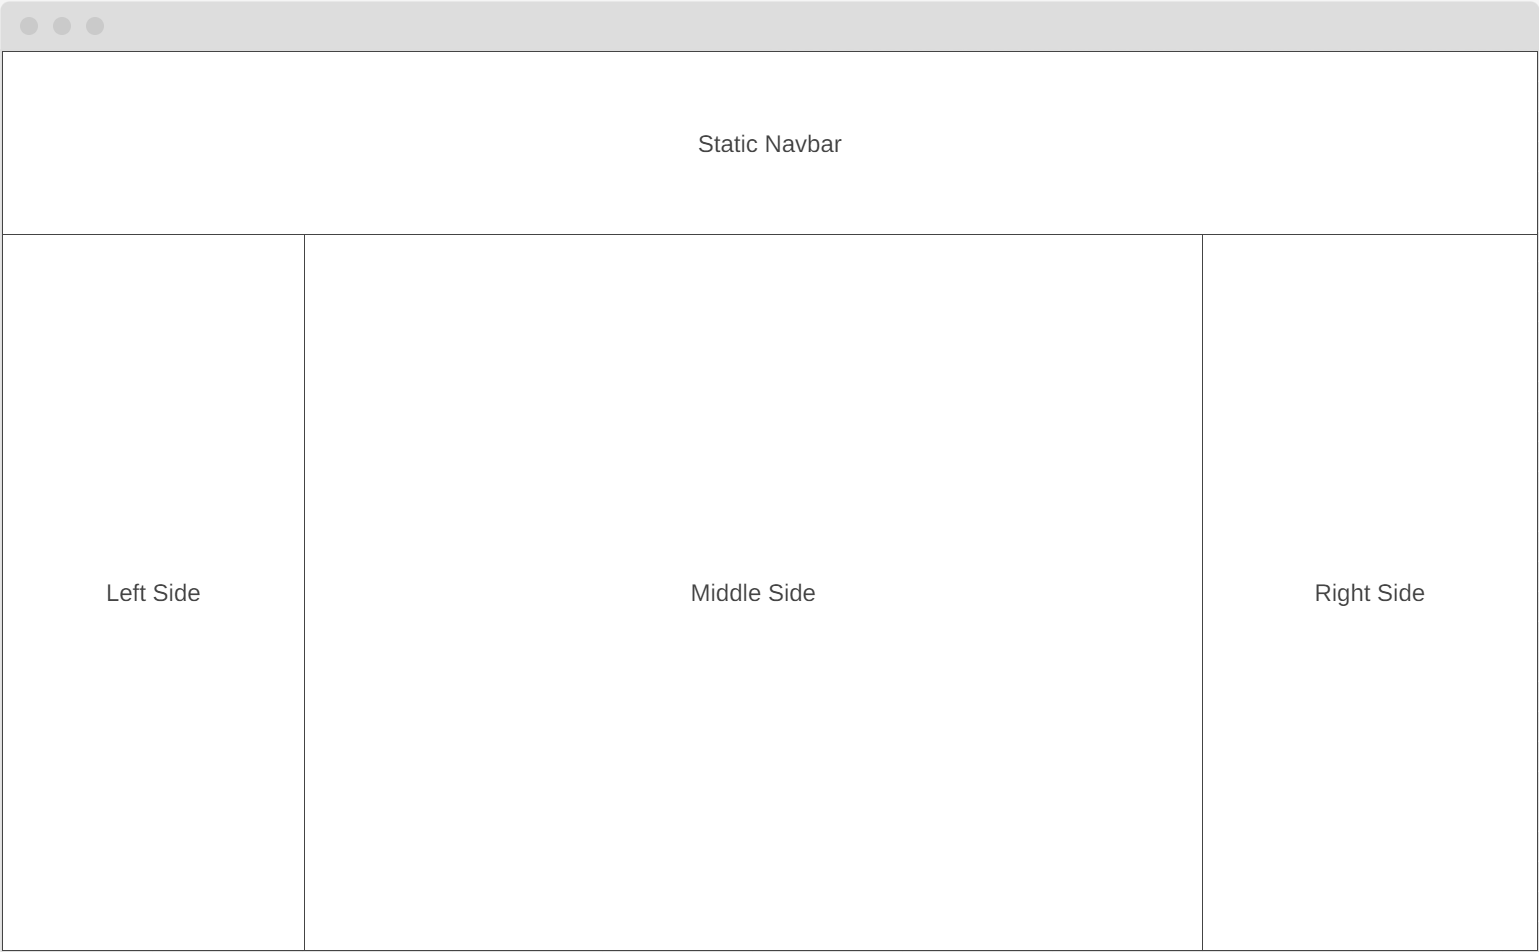
\includegraphics[scale=0.6]{images/courses-layout.png}
  \caption{Courses Module Layout - Desktop}
  \label{fig:figure10}
\end{figure}

\subsection{Search}

\noindent The search page is used for course navigation, presenting a general list of courses and the possibility to search through them. How the search input is parsed to produce the returned list of courses is explained in the backend chapter. In this subsection, the presented information for the user is explained. The components presented below can be seen in Figure \ref{fig:search-page}.
\\\\
\noindent Courses are displayed to the user in the format of cards. A course card consists of the title and subtitle, with the course description and the course tags. This information should be enough for identifying the course, and more details about it can be obtained by clicking it, which will open the course view. There is a height limit put on the description, so in case it gets exceeded, the content will become scrollable.
\\\\
\noindent The card also contains a search score when the search input is not empty. The score represents how likely the course is what the user was searching for. Although it theoretically is a score between 0 and 100, a 100 score is impossible, since you would need to search for everything present in the course to get it. The score is still relevant through relativity, as it can be used to order courses from the search. The course that has the higher score in a search is most likely more relevant than one with a lower score.
\\\\
\noindent While the middle side contains the search bar and the list of courses, the right sidebar contains a search history. Currently, the search history is saved inside \textbf{localStorage} and has a maximum of 10 entries. Older entries are automatically removed. All entries can, in fact, be removed through a clear all button that will empty the search.
\\\\
\noindent The search history is updated on each input change from the search field, but to avoid updating the history on each letter change, the \textbf{useDebounceCallback} hook from \textit{usehooks-ts} is used \cite{usehooks-ts}. The hook waits for half a second before signaling the input value change. If in the meantime a new value change event is triggered, then the waiting event is canceled, and the new event will also begin to wait. Eventually, the wait finishes without other events being triggered, and that is when the callback that has been waiting finally executes.
\\\\
\noindent In case there are no search results or the search history is empty a proper message is shown so the user is aware it is in fact not a loading error or broken display, and indeed there was nothing to show for their input. 

\begin{figure}[h]
    \centering
    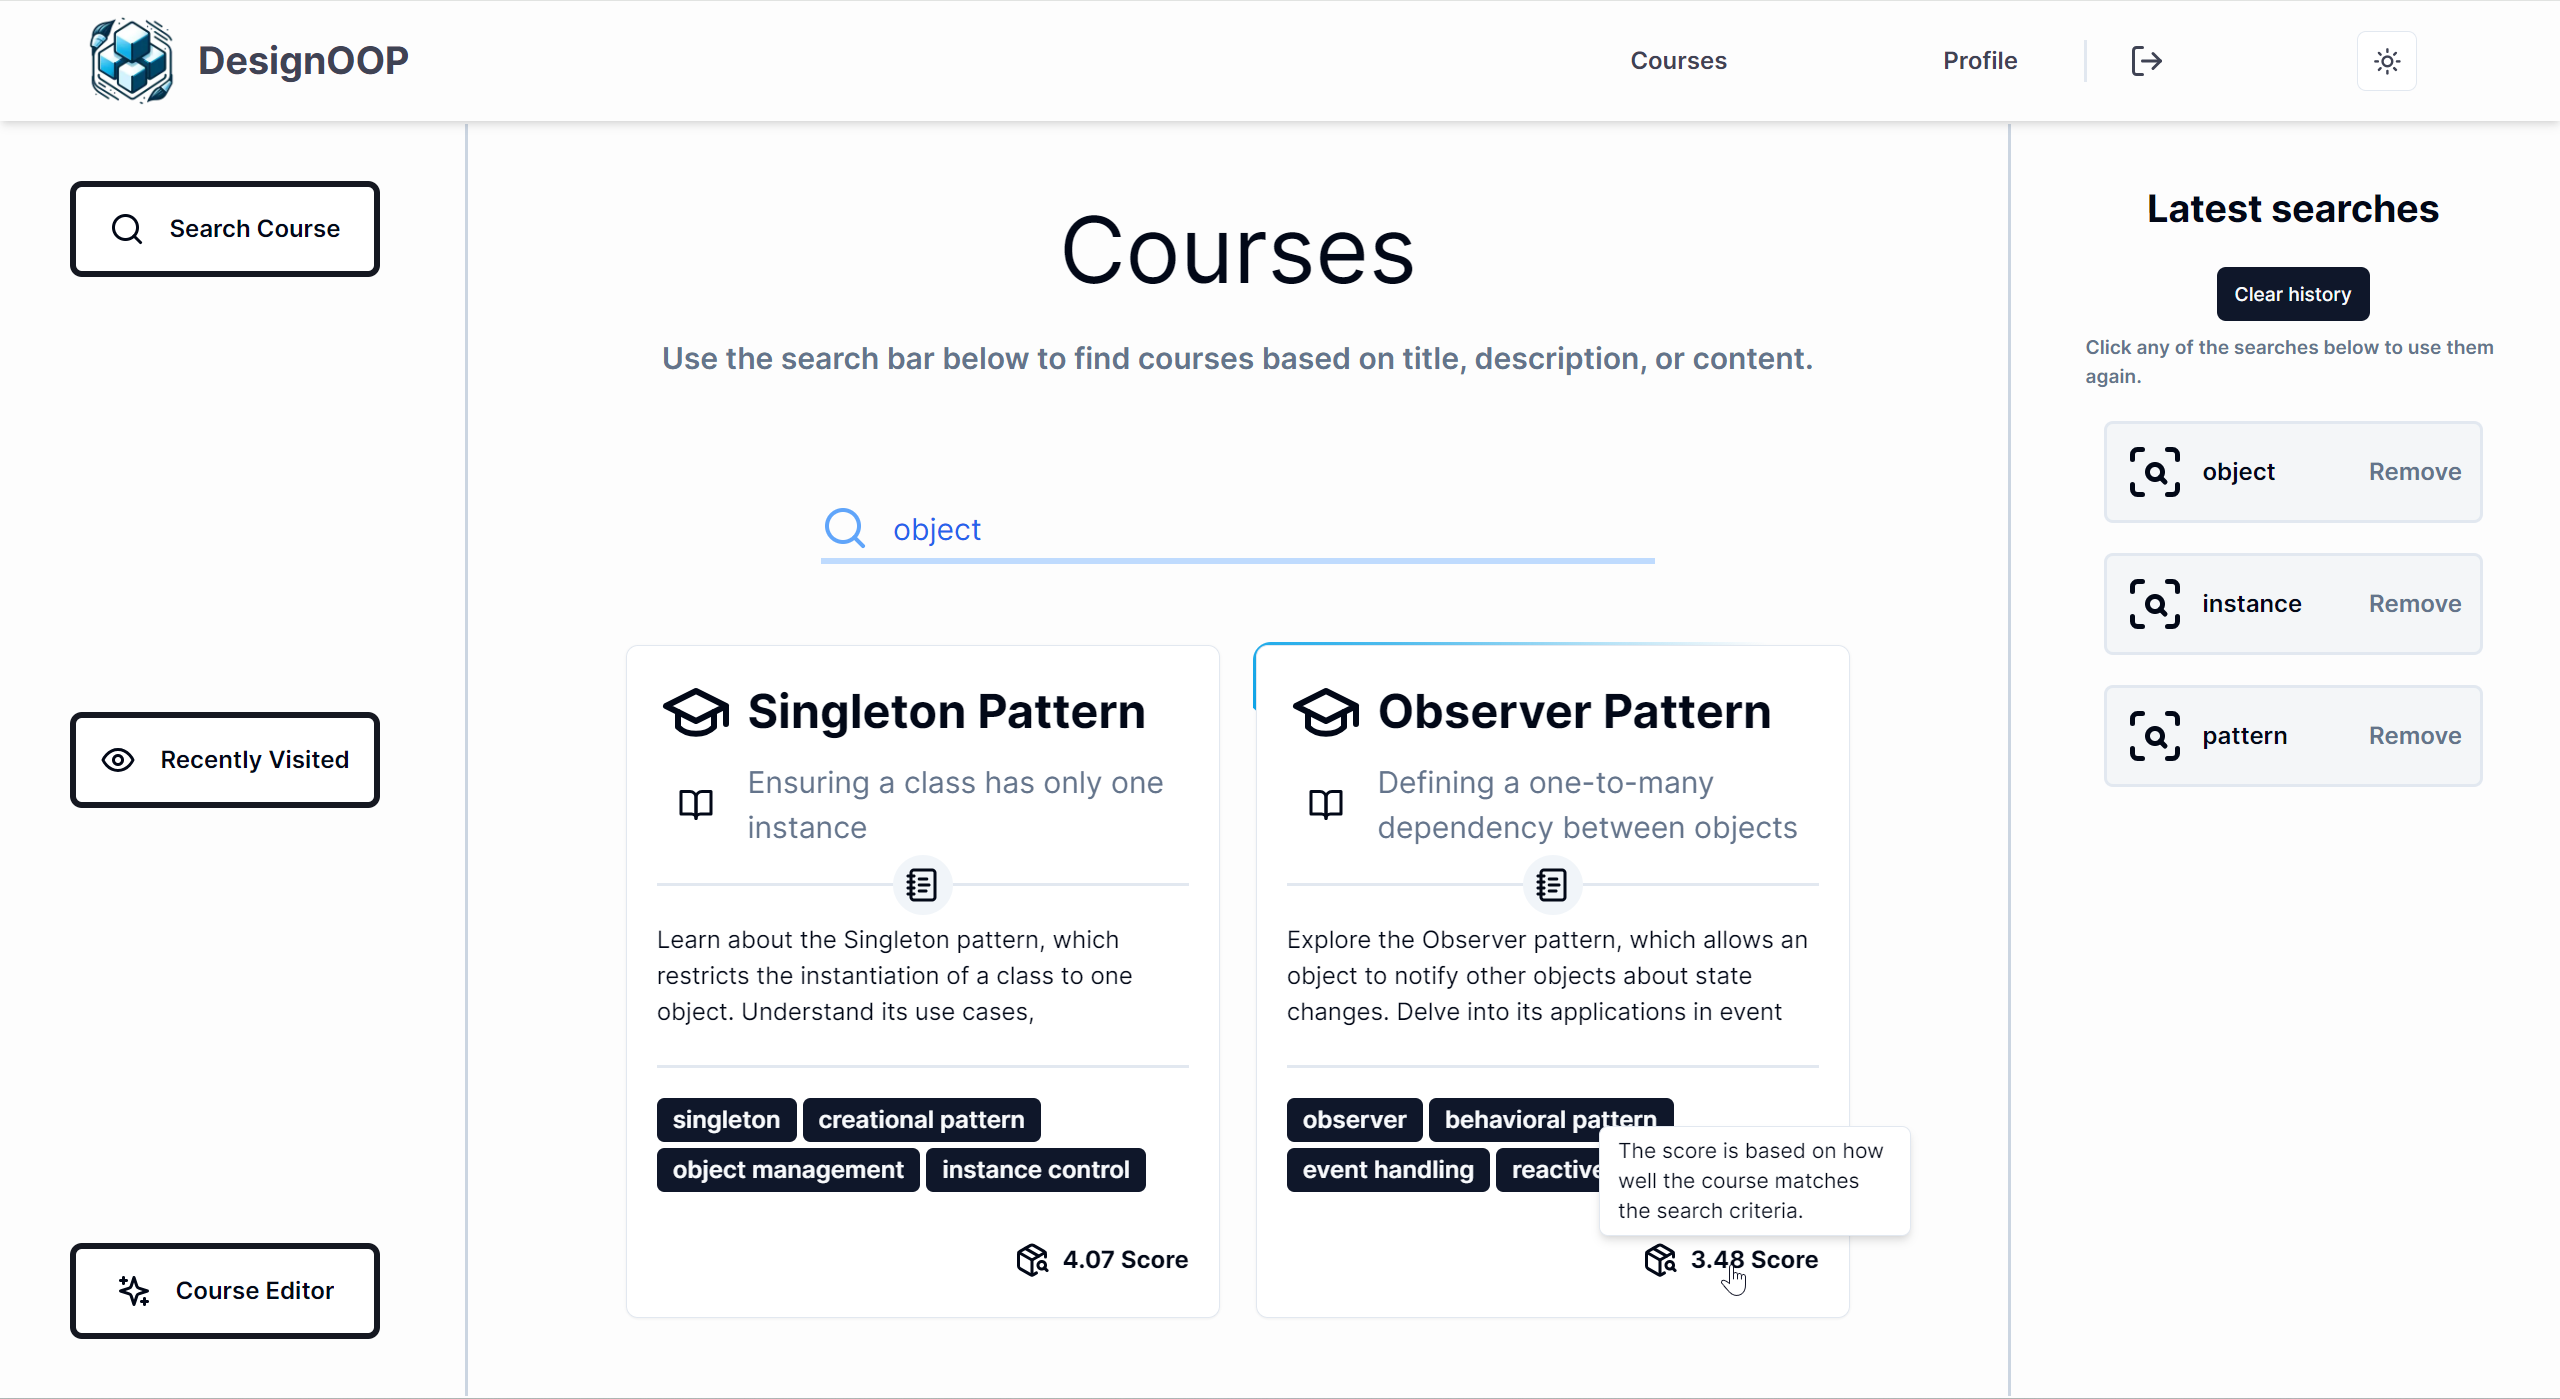
\includegraphics[scale=0.33]{images/search-page-preview.png}
    \caption{Courses search page}
    \label{fig:search-page}
\end{figure}

\subsection{Browsing History}

\noindent The course browsing history is also stored inside the \textbf{localStorage}. When entering a course page, a component used specially for side effects named \textbf{CourseViewHistory} uses the \textbf{useLocalStorage} hook from \textit{usehooks-ts} to update the browsing history of the \textbf{localStorage}. To avoid trips to the database, the information needed to output the course inside the history is saved completely.
\\\\
\noindent A \textbf{CourseHistoryItem} refers to the information needed to display a visited course. It contains the same information as a course card from the \textbf{Search} subsection, to which the search score is replaced with a last visited date. Since the course card is saved fully, even if the course information changes or is deleted, the display at which the course was accessed will be preserved.
\\\\
\noindent While the middle side displays the history, the right side presents the user with extra actions that they could take regarding it. Currently, the user can only clear their browsing history, but in the future, course recommendations might be placed here as well.
\\\\
\noindent When the browsing history is empty, a message telling the user that the page will be populated after some courses are accessed is displayed.

\begin{figure}[h]
    \centering
    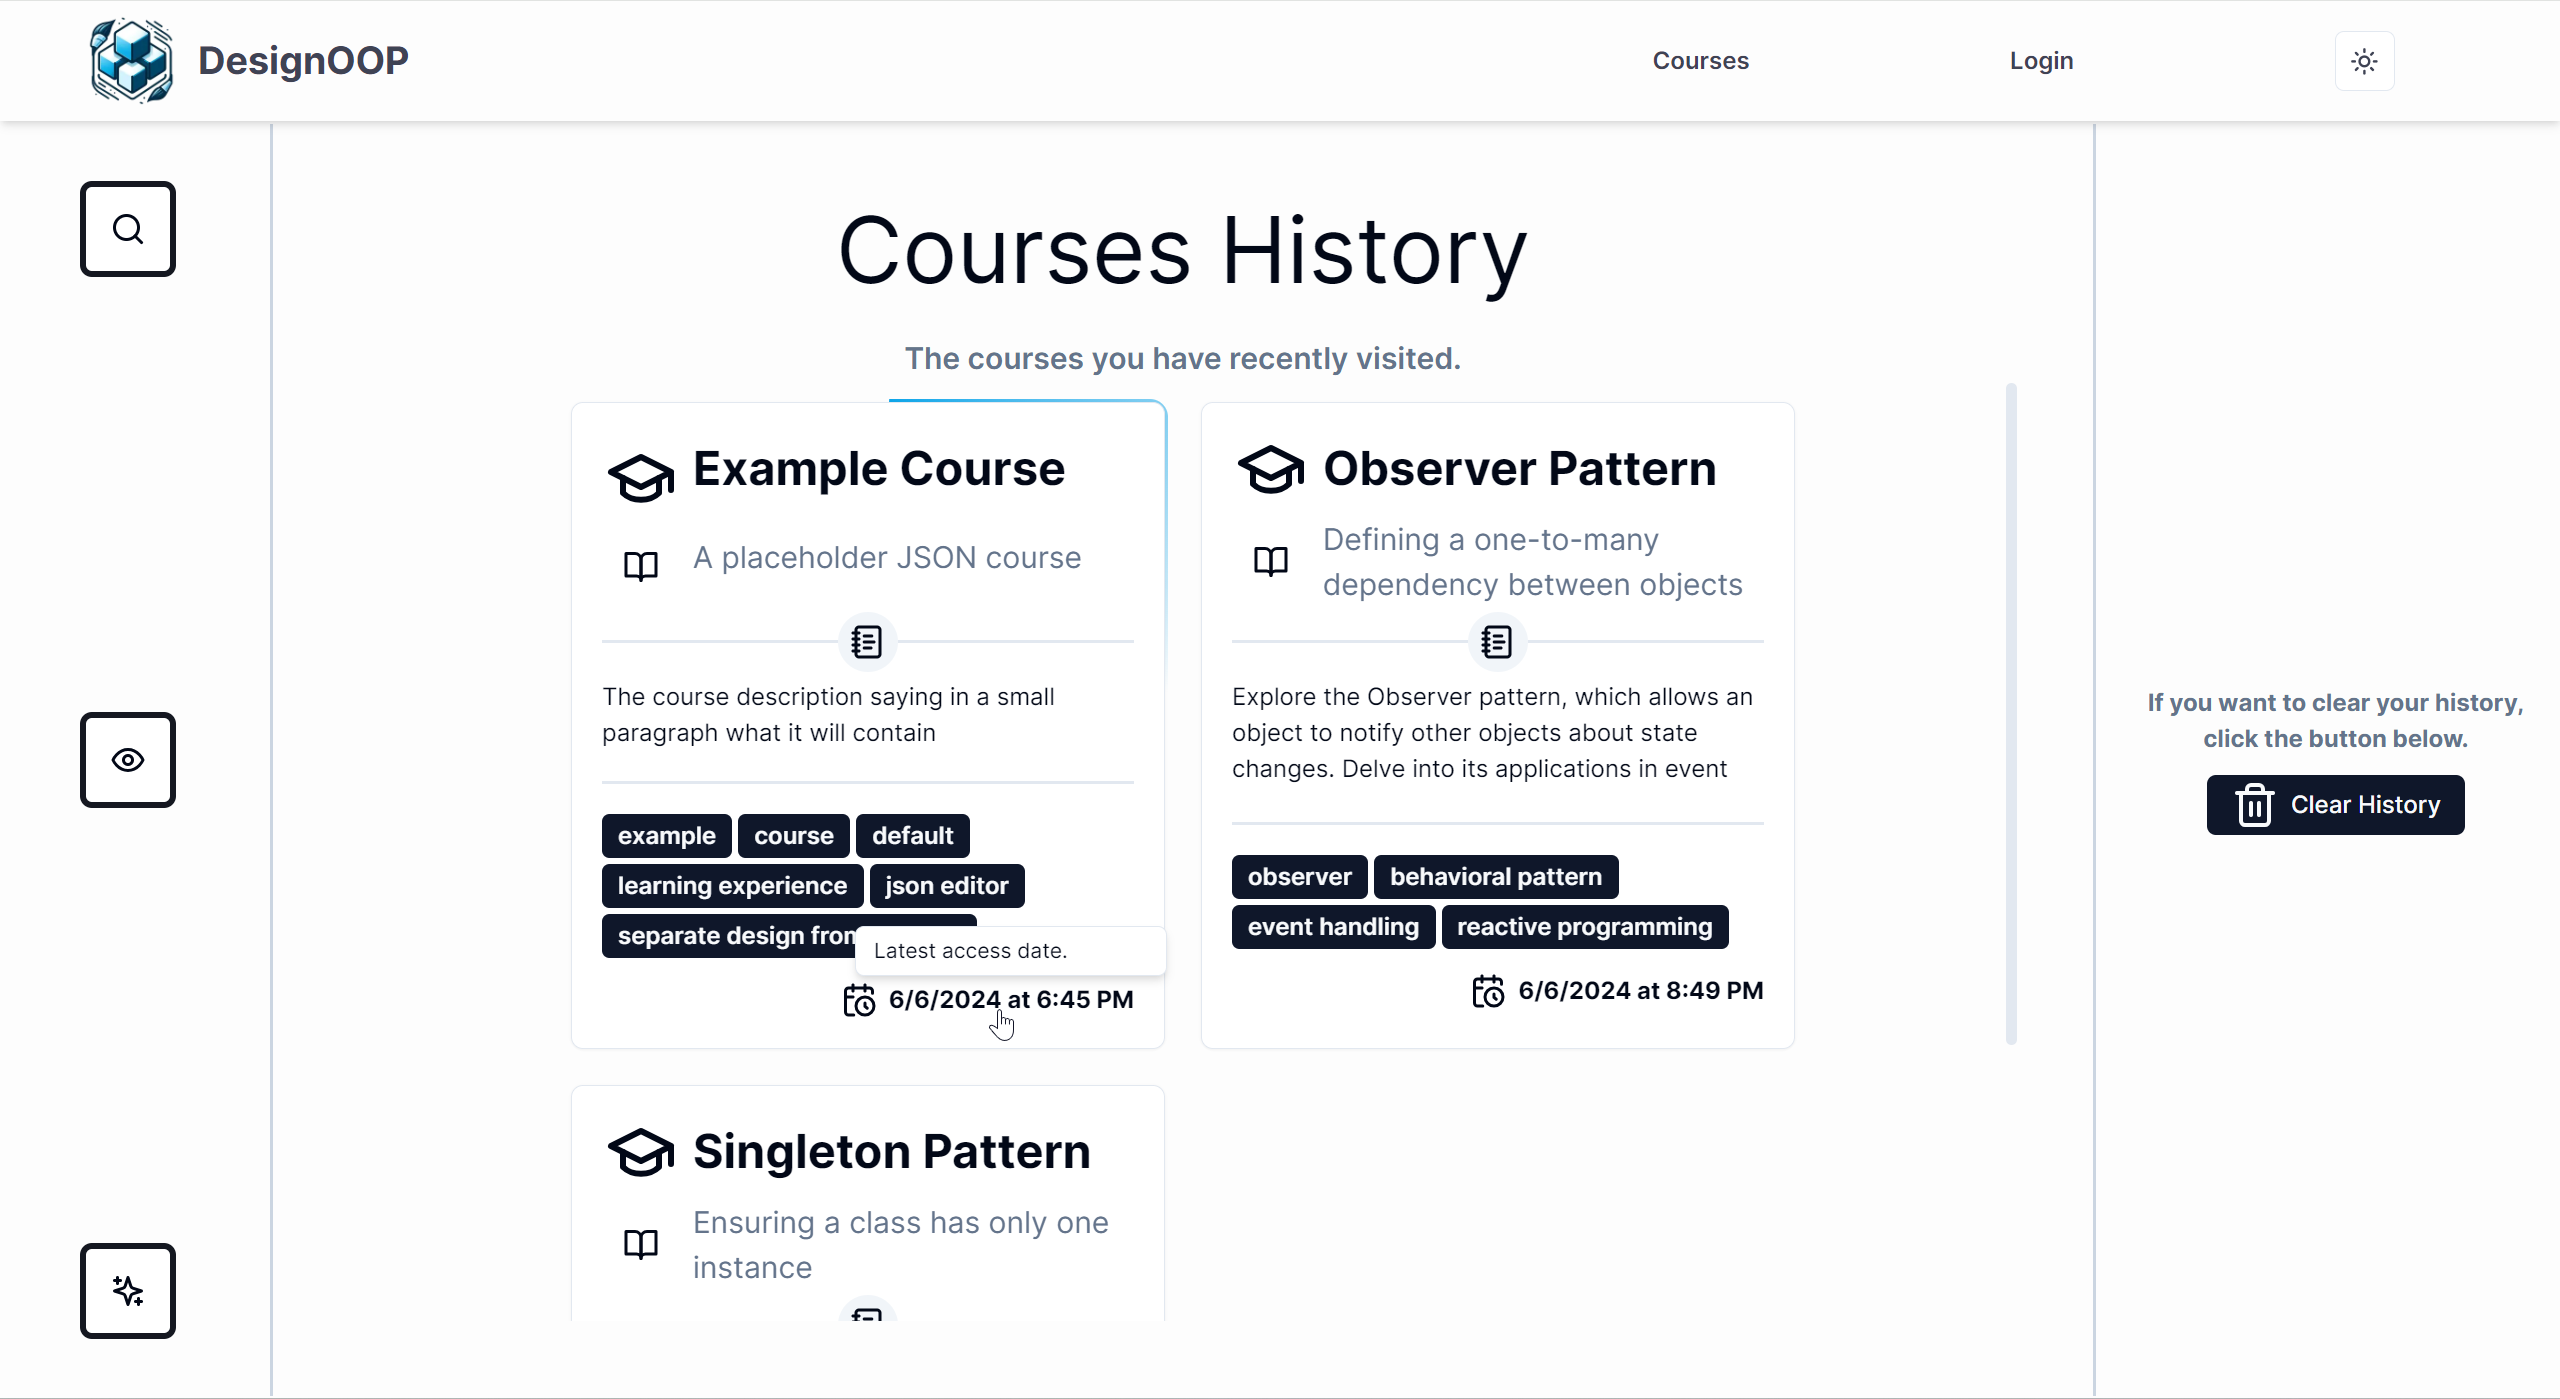
\includegraphics[scale=0.33]{images/courses-history.png}
    \caption{Courses browsing history page}
    \label{fig:courses-history}
\end{figure}

\subsection{View}

\noindent The course view loads the course in the middle section and utilities in the right side, such as a table of contents that helps navigation through the course's components (see Figure \ref{fig:course-table-of-contents}). Besides the table of contents, user actions are declared on the right side. Based on the authorization of the user, the actions could include a delete course button. To ensure it was not clicked by accident, a dialog will open that asks the user to type the name of the course to confirm deletion. Regardless of user authorization, a button for opening the course inside the course editor is shown to encourage users to create their own resources and learn from already written examples.
\\\\
\noindent In case the course can't load due to reasons such as an invalid courseId format, course not found, or unknown errors, the middle and right sides will display an appropriate error message.

\begin{figure}[h]
    \centering
    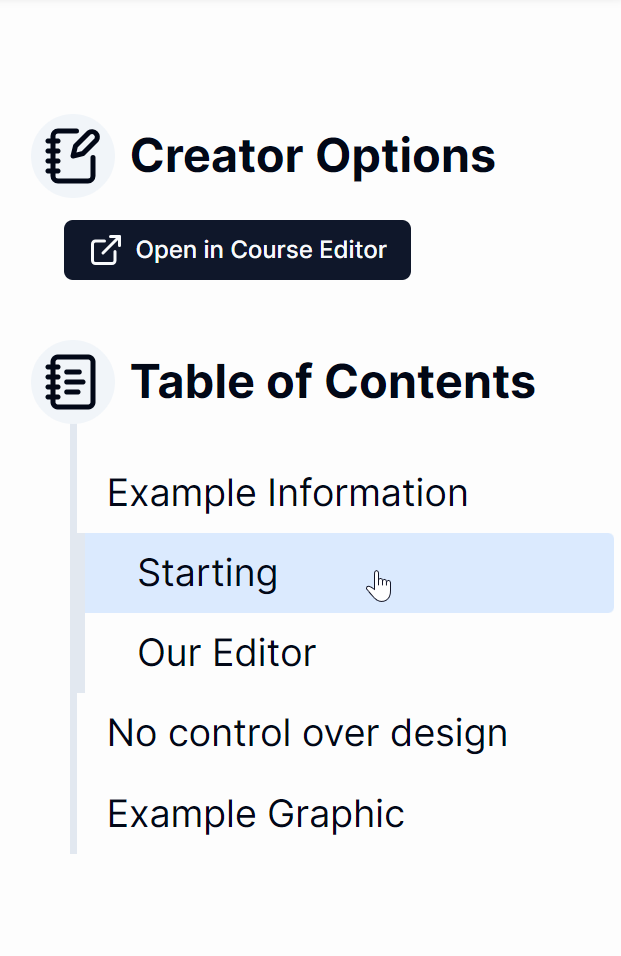
\includegraphics[scale=0.7]{images/table-of-contents.png}
    \caption{Course View - Right Side}
    \label{fig:course-table-of-contents}
\end{figure}

\section{Course Editor}

Although the course content is kept separate from the design, its internal structure can get very complex and intricate. Editing it in a usual text or code editor might prove challenging, as the most you can get out of them is syntax highlighting for JSON and autocompletion of brackets. For this reason, the web platform implements its own editor tool that can help the creator in a more specific way.

\subsection{Course Structure}

\noindent A \textbf{Course} component will parse the metadata of the course, along with the components tree, which is recursively parsed by \textbf{DynamicCourseComponent}.
\\\\
\noindent The \textbf{components} property of the course consists of multiple objects that can have dynamic parameters. For identifying them, all components must have the \textbf{componentType} property. In a separate \textbf{dynamic-course-components.tsx} file located inside the \hl{@/modules/courses/constants} folder, a \texttt{Components} constant object is declared. This constant maps a string to a configuration that contains three properties: \textbf{component}, \textbf{params}, and \textbf{hasChildren}. The \textbf{component} property returns a React component. The string that maps to this configuration is none other than the value of the \textbf{componentType} property.
\\\\
\noindent After the component configuration is identified using the raw JSON object, the \textbf{DynamicCourseComponent} will take the other properties of the object, with the exception of the \textbf{children} and \textbf{contentTable} properties, and pass them as parameters to the React component from the configuration. Using \texttt{useMemo}, the \textbf{children} property is parsed into a list of more dynamic components, therefore creating the recursive part. The usage of this hook ensures that the children are not rendered again unless the JSON object changes.
\\\\
\noindent All course components can be found inside the \hl{@/modules/courses/components/course/components} folder. If a new component is created or the parameters are modified, the \texttt{Components} constant also needs to be modified to reflect the changes.
\\\\
\noindent Each dynamic component is wrapped into an \textbf{ErrorBoundary} component, which will try to catch rendering errors as soon as they appear. This is especially useful in mid-editing, when components might not be written properly but you still want to be able to see the parts that work. The \textbf{ErrorBoundary} simply replaces the content with an error message.

\subsection{JSON Editor}

\noindent The JSON Editor is meant to fit the role of a code editor, specialized for creating resources that respect the format of this web platform. To achieve this, the \textbf{CodeMirror} library \cite{codemirror} was used. Since it is a JavaScript component, it cannot be used directly in React, as it needs to be wrapped inside a component. To do this, the web platform uses an already existing React wrapper over CodeMirror, \textbf{react-codemirror} by uiw \cite{react-codemirror}.

\begin{figure}[h]
    \centering
    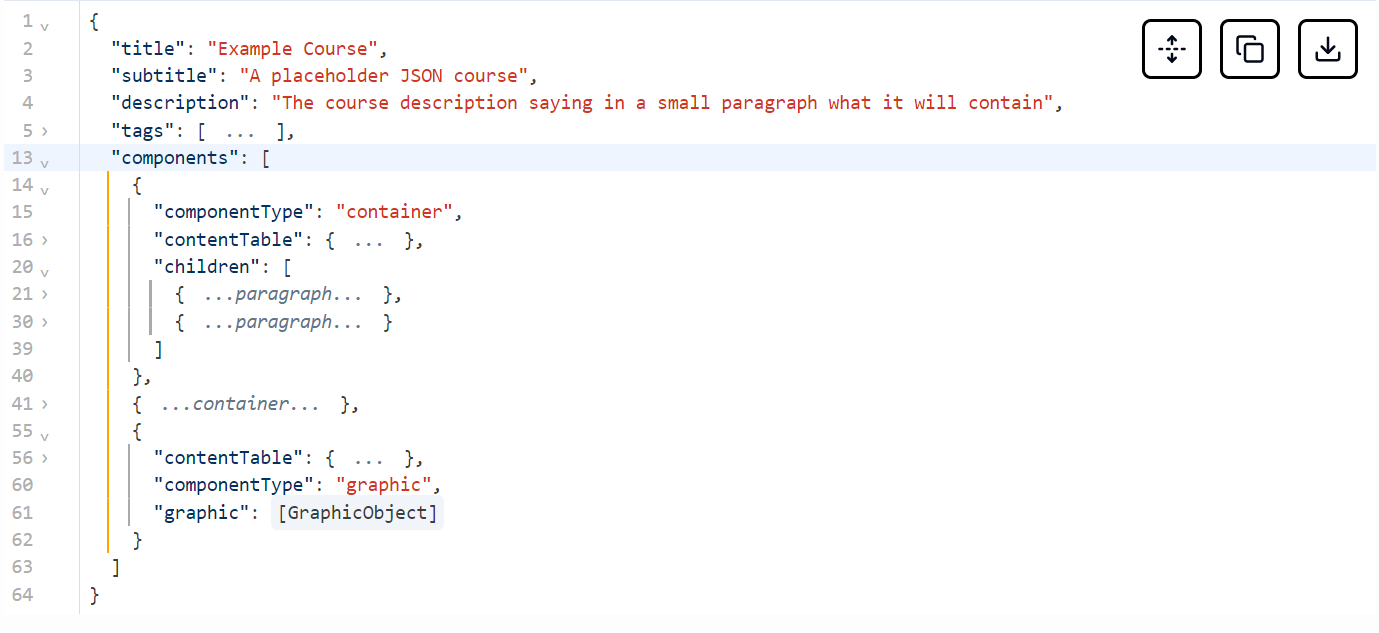
\includegraphics[scale=0.63]{images/json-editor-light.png}
    \caption{JSON Editor with example course - Light Theme}
    \label{fig:json-editor-light}
\end{figure}

\begin{figure}[h]
    \centering
    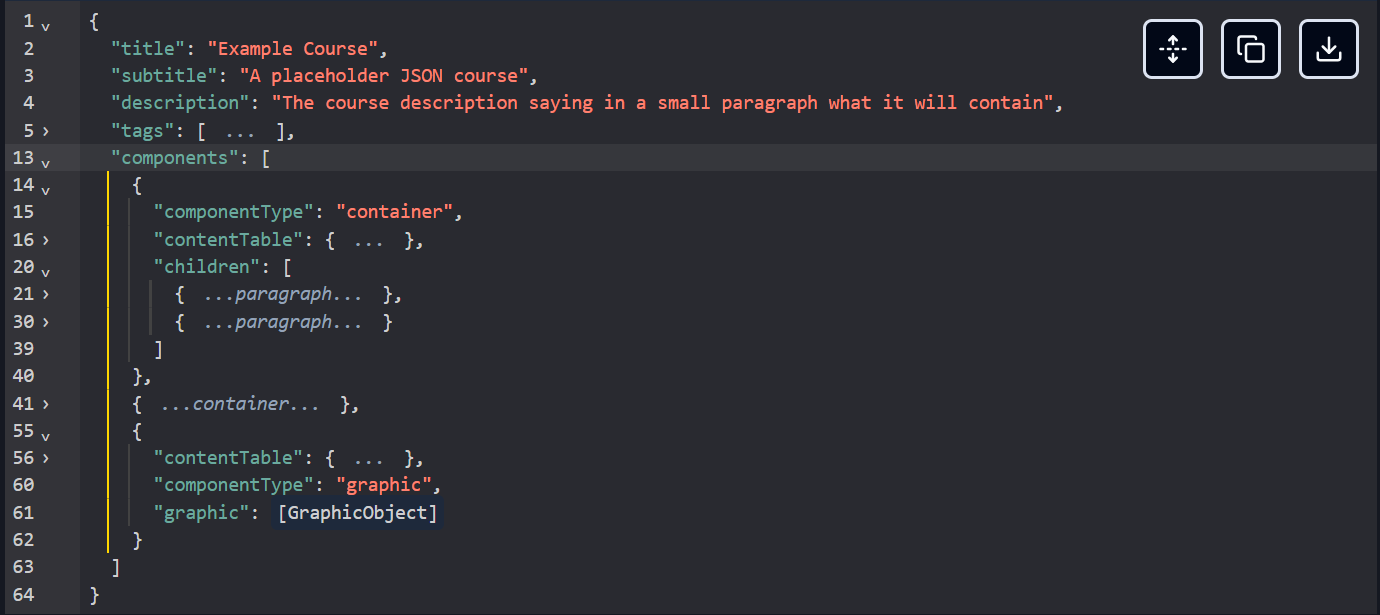
\includegraphics[scale=0.63]{images/json-editor-dark.png}
    \caption{JSON Editor with example course - Dark Theme}
    \label{fig:json-editor-dark}
\end{figure}
\newpage
\noindent The JSONEditor component is responsible for bringing together all the custom features that make the code editor functional. Firstly, it returns a react CodeMirror instance, to which a JSON content is passed as initial value. For syntax highlighting, the \texttt{lang} parameter is set to "json". The CodeMirror component also receives several more parameters, such as a theme, a list of extensions, an \texttt{onUpdate} function and a ref object that is later used for external access to the state via utility buttons.
\\\\
\noindent To synchronize the \textbf{theme of the editor} with the theme of the web platform, the \texttt{xcodeLight} (visible in Figure \ref{fig:json-editor-light}) and \texttt{xcodeDark} (visible in Figure \ref{fig:json-editor-dark}) themes are imported from the \texttt{@uiw/codemirror-theme-xcode} package and used according to the theme from next-themes. To choose between the themes, the \textbf{resolved theme} provided by the \texttt{useTheme} hook is used.
\\\\
\noindent Three utility buttons are displayed in the right corner of the editor (also visible in Figure \ref{fig:json-editor-light}). The first button, \textbf{Folding toggle}, uses the syntax of the code inside the editor to either collapse all blocks or expand them. When components are collapsed, the JSON editor will display a widget \textbf{"...componentType..."}. In a hierarchy this can be useful for visualizing the tree depth without unnecessary code reveals or nameless collapsed blocks that don't offer any information. The second button, \textbf{"Copy to clipboard"}, is a classic usage button that allows you to quickly retrieve the information from the editor inside your clipboard. The third button, \textbf{Download JSON}, is used for downloading the content inside a \texttt{course.json} file. This is useful when the content gets very long, and you want to save local copies of your work.
\\\\
\noindent The \textbf{onUpdate} function receives a \texttt{viewUpdate} as a parameter when triggered. This \texttt{viewUpdate} contains details regarding the modifications of the code view. \textbf{Attention!} This does not only refer to state modifications but includes fine-grained details such as cursor position changes, linter suggestion additions, hovering over warnings, and so on. Although this much access to detail is great, it is unnecessary for the use case of saving the new JSON after it gets updated. To filter the unnecessary monitored changes, a custom function is used that checks the transactions within the update. To pass the filter, the update needs to have an effect of type \textbf{setDiagnosticsEffect} inside it. This ensures that the update function after the filter will have access to the latest diagnostics, as there is a delay between the actual change of the document and the setting of diagnostics, but it is known that the diagnostics trigger on each document change. A further optimization is done by the usage of \textbf{useDebounceCallback} on the update function, which limits the update function from triggering at most once per half a second.
\\\\
\noindent The editor provided by CodeMirror benefits from a lot of extension points. Some of them that are more complex, such as linting and autocompletion, are discussed in the following subsections, while the simple ones are explained here.
\\\\
\noindent The \textbf{graphicWidgets} is a custom implemented extension that can be found inside the \texttt{@/modules/courses/utils/json-graphic-replace.tsx} file. A graphic component parsed as a JSON object contains a very long base64 string, that if left unformatted will occupy too much of the editor's screen. To avoid this, an extension that parses the \textbf{"graphic"} property is implemented. This extension replaces the long base64 string with a special widget called \textbf{[GraphicObject]} (visible on line 61 inside the Figure \ref{fig:json-editor-light}). This only happens if the graphic property's value starts with a dot. This is done just in case the user would like to keep the long string visible for whatever reasons. The widget is not a simple label though, as it is also clickable. When clicked, the widget will open a \textbf{toast} message at the top of the page, with two possible actions: \textbf{Open in editor} and \textbf{Set graphic from clipboard}. The first option will open the graphic editor with the graphic that is hidden by the widget parsed inside the editor. The second option will assume you have a graphic in your clipboard, and replace the one behind the widget with the new retrieved one.
\\\\
\noindent The \textbf{lintGutter} extension is imported from the \texttt{@codemirror/lint} package and is responsible for adding decorations to the gutter of the code editor. For example, a red dot will appear for lines with errors and a triangle for lines with warnings.
\\\\
\noindent The \textbf{indentationMarkers} extension, imported from \textbf{@replit/codemirror-indentation-markers} package is responsible for adding vertical lines to the indentation of the JSON. These lines are helpful since the components might become very intricate, and it is important to be able to easily differentiate between depth levels. You can also better interpret your position in the document, as the depth level that you are at is highlighted with a different color than the other lines.
\\\\
\noindent A JSON line can get very long when writing properties such as descriptions or paragraphs. To avoid horizontal scrolling for these lines, the editor is using two extensions for line wrapping. Firstly, \textbf{EditorView.lineWrapping}, where \texttt{EditorView} is imported from \texttt{@codemirror/view}, is an extension that wraps lines when their length exceeds the editor's. Secondly, \textbf{wrappedLineIndent} from the \texttt{codemirror-wrapped-line-indent} package is an extension responsible for keeping the depth level of the property when line wraps.

\subsection{Custom JSON Parser and Grammar}

\noindent Although the course content can be parsed as a normal JSON, to facilitate linting and autocomplete, that make use of the syntax tree, the JSON grammar is extended, with custom properties that will help easier map the components.
\\\\
\noindent When thinking about the customization of suggestions and linting of the course JSON, two strategies were considered.
\\\\
\noindent The first option, keeping the logic private inside the backend was considered a good solution for multiple reasons. It takes the computational load away from the client browser, as the heavy operations are handled by the backend server. If there is some logic that the client should not know, it can safely run in the backend, so it is also good for protecting business logic.
\\\\
\noindent Since the focus at this point was the backend, technologies such as \textbf{ANTLR4 (ANother Tool for Language Recognition v4)} have been considered and a language server strategy to be employed was chosen. ANTLR helps generating a parser based on a grammar, and also has Java integrations, which makes it a good choice for the Spring Boot backend. \textbf{Language servers} have a defined standard for the request and response, which allows them to easily connect with multiple applications that implement the same standard. For more details regarding this method, check \cite{language-server-protocol}. This would mean that not only the syntax tree will be produced by the backend, but the diagnostics and autocomplete suggestions as well. \textbf{CodeMirror} also seemed to have integration endpoints for language server as well, so it would have been relatively easy to utilize it.
\\\\
\noindent Although this approach has benefits, there are two downsides to it that were considered as well. Firstly, the trade-off between privacy and speed. Although the computational load is moved elsewhere, making the request and waiting for the response will also delay the whole process. Besides that, a considerable downside is the fact that the editor is now dependent of a server, and won't be able to process the syntax tree without it.
\\\\
\noindent With the previous considerations in mind, the choice to have the parser on the client side was made. In this way, the user could use the editor even without access to internet. Looking through CodeMirror's forum and documentation, a JavaScript parser system that directly integrates in the browser and has CodeMirror compatibility, since it is maintained by the CodeMirror team, was found. \textbf{Lezer} \cite{lezer} is an open source library that provides a parser generator which outputs JavaScript modules.
\\\\
\noindent The grammar for the JSON parser is defined in the \texttt{json.grammar} file, located inside the \hl{@/modules/courses/utils/lezer-parser} folder. The grammar is written in a custom format that is later parsed by the \texttt{lezer-generator} package. The \texttt{lezer-generator} package is a command line tool that generates a JavaScript module from the grammar file. To create the \textbf{lezer-parser.ts} and \textbf{lezer-parser.terms.ts} files, the command \hl{npx lezer-generator json.grammar -o lezer-parser.ts} is executed. The \textbf{lezer-parser.ts} file contains the parser, while the \textbf{lezer-parser.terms.ts} file contains the terms used in it.
\\\\
\noindent The grammar was obtained by using an existing JSON one, taken from the \textbf{@lezer/json} package, and extending it with custom properties. The customization had to be as abstract as possible, as adding syntax for each component would be inefficient since the parser would need to be updated each time a new component is added. The custom properties added to the JSON grammar are \textbf{componentType}, \textbf{graphic}, \textbf{children}, and \textbf{contentTable}. The \textbf{componentType} property is mandatory for all components, as it is used to identify the component. The \textbf{graphic} property is used to hide long base64 strings behind a widget. The \textbf{children} property is used to create a recursive structure of components. The \textbf{contentTable} property is used to create a table of contents for the course view. To test the new grammar, an existing playground was used, which is available at \cite{lezer-playground}.

\begin{figure}[h]
    \centering
    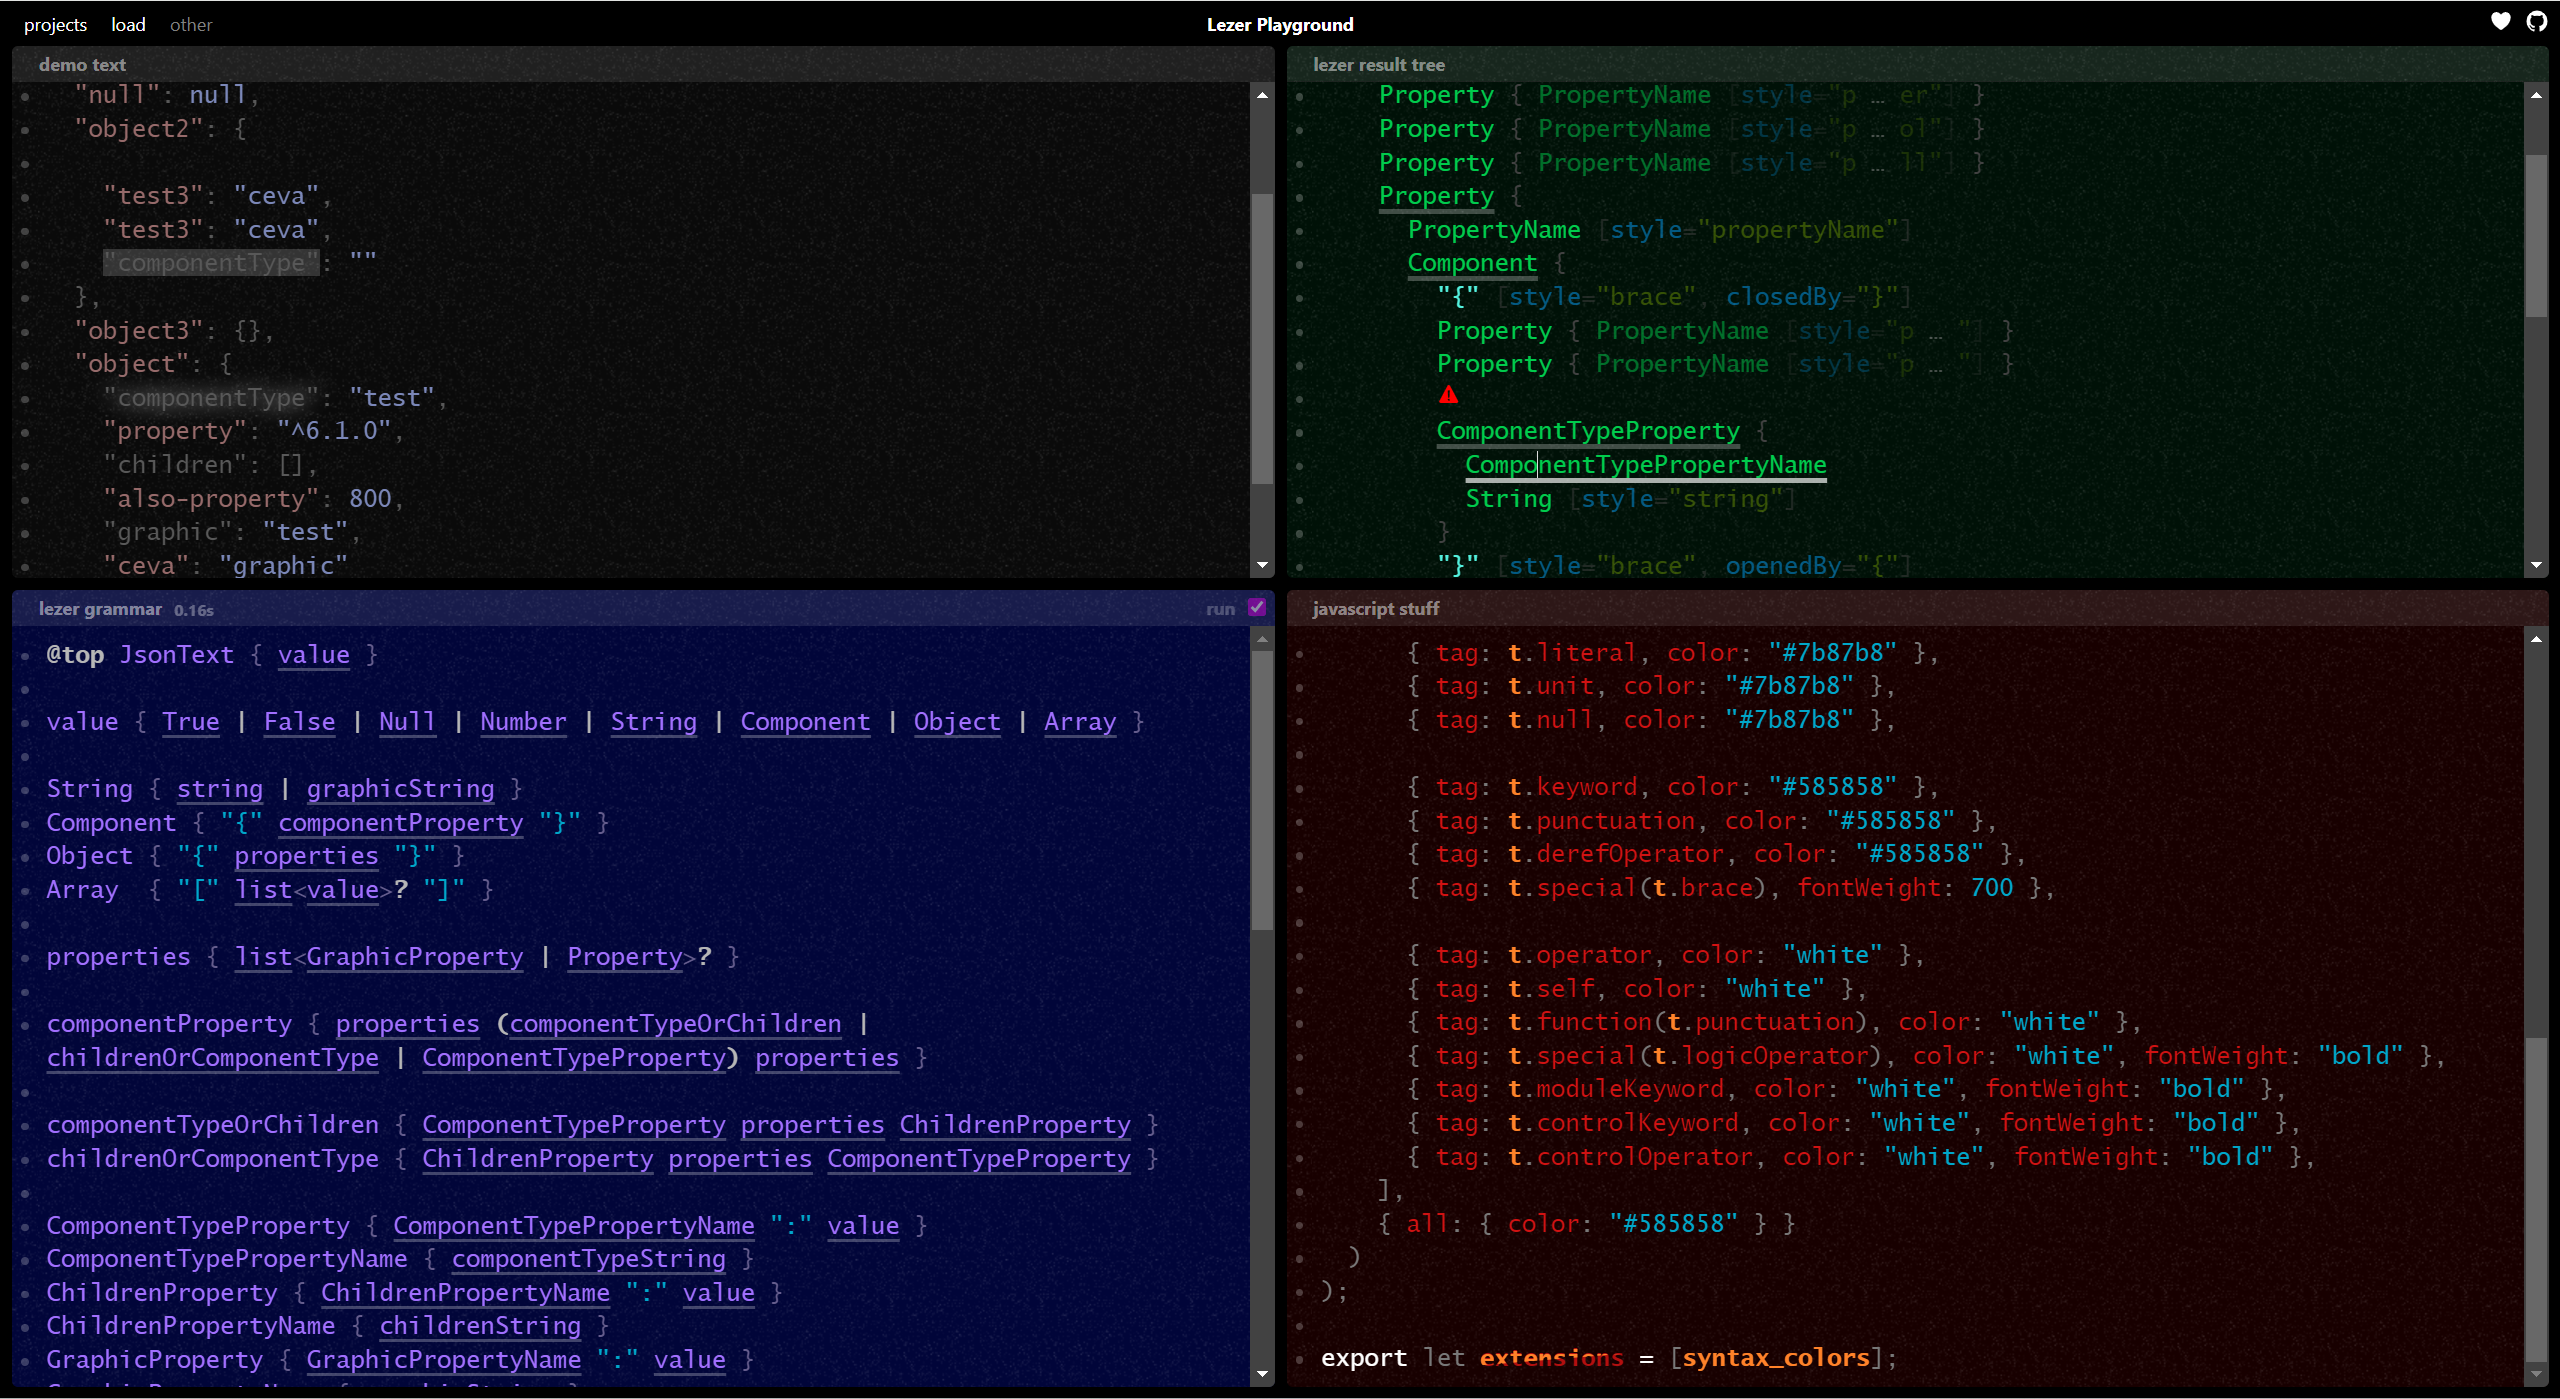
\includegraphics[scale=0.35]{images/lezer-playground.png}
    \caption{Grammar test in the Lezer playground \cite{lezer-playground}}
    \label{fig:lezer-playground}
\end{figure}

\noindent The previously obtained parser is used to create a language extension for the CodeMirror editor. This is done inside the \textbf{json-course-language.ts} file, located inside the \hl{@/modules/courses/utils} folder. Now that the parser has been encapsulated in a \textbf{LanguageSupport} object, it can be used directly in the extensions list.

\subsection{Linting}

\noindent Since Components are defined with a configuration that contains parameters information, those can be used to offer personalized linting messages. Warnings are provided when a component is missing a mandatory parameter, or when a parameter is not of the correct type. The linting messages are displayed in the gutter of the editor. 
\\\\
\noindent Without a custom syntax tree, to identify the type of the component and its children, the linter would need to parse the JSON content and analyze it. This would be a very heavy operation, especially for large JSON files. To avoid this, the custom syntax tree is used, which is generated by the Lezer parser. The linter can now easily identify the type of the component and its children, by using search based on the custom properties added to the JSON grammar.
\\\\
Although the current grammar is not very complex and doesn't add a lot of optimization, it is a good start for future improvements. The linter can be extended to offer more personalized messages or there could be multiple grammars that map different languages to the same syntax tree, which would allow the linter to be used for multiple languages.
\\\\
\noindent If linter errors are identified, the editor will display a red dot in the gutter, and the line with the error will be highlighted. Hovering over the red dot will display the error message (see Figure \ref{fig:json-editor-linter-error}). While errors are present, the content of the editor will not replace the JSON content of the course, as the user might not be aware of the error. The user will be able to save the content only after the errors are fixed.

\begin{figure}[h]
    \centering
    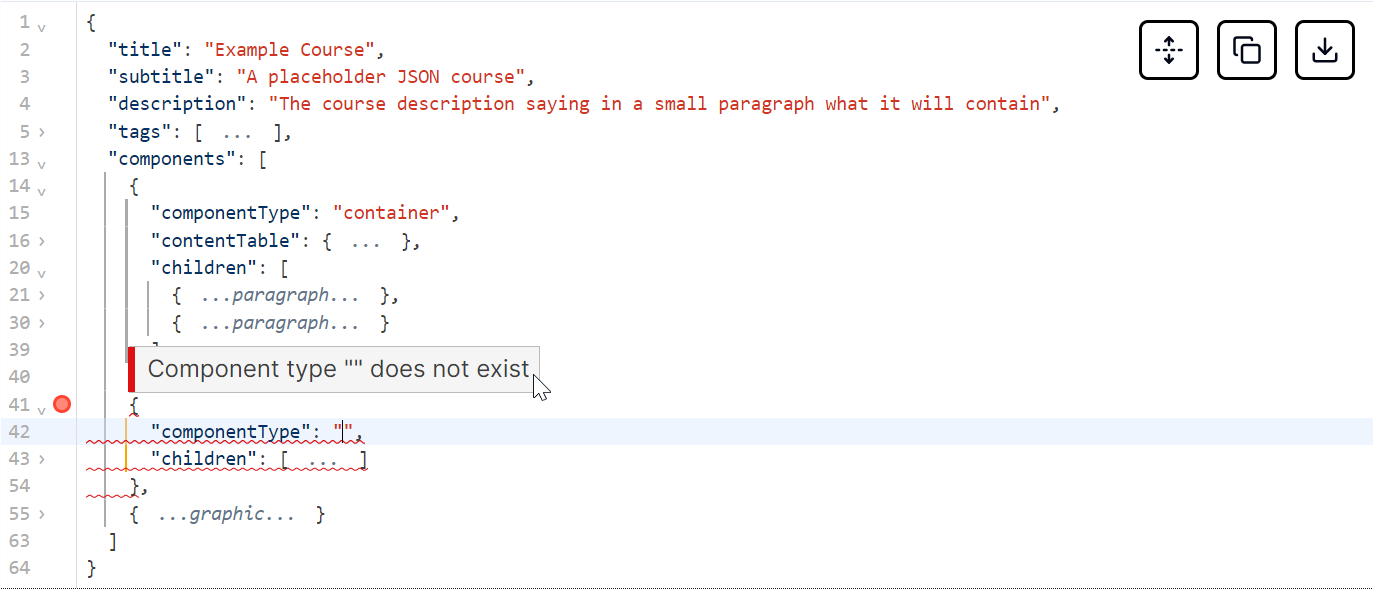
\includegraphics[scale=0.62]{images/json-editor-linter-error.png}
    \caption{JSON Editor - Linter Error Example}
    \label{fig:json-editor-linter-error}
\end{figure}

\subsection{Autocomplete}

\noindent There are two types of autocompletion that are implemented in the JSON editor. The first one is the autocompletion of the components (see Figure \ref{fig:json-editor-autocomplete-components}). When typing a componentType inside the components/children property, a list of components will be displayed. The second one is the autocompletion of the parameters (see Figure \ref{fig:json-editor-autocomplete-fields}). When typing a parameter inside a component, a list of parameters will be displayed. The parameters are filtered based on the componentType that is being typed.
\\\\
\noindent After a suggestion offered by the CodeMirror editor is selected from the list of suggestions generated by the custom extensions \textbf{json-autocomplete-components.ts} and \textbf{json-autocomplete-parameters.ts}, it will be inserted inside the editor at the cursor position. The code snippet that gets inserted might contain placeholders for values, which can be navigated through by pressing the tab key. The placeholders are replaced with the actual value when the user types something.

\begin{figure}[h]
    \centering
    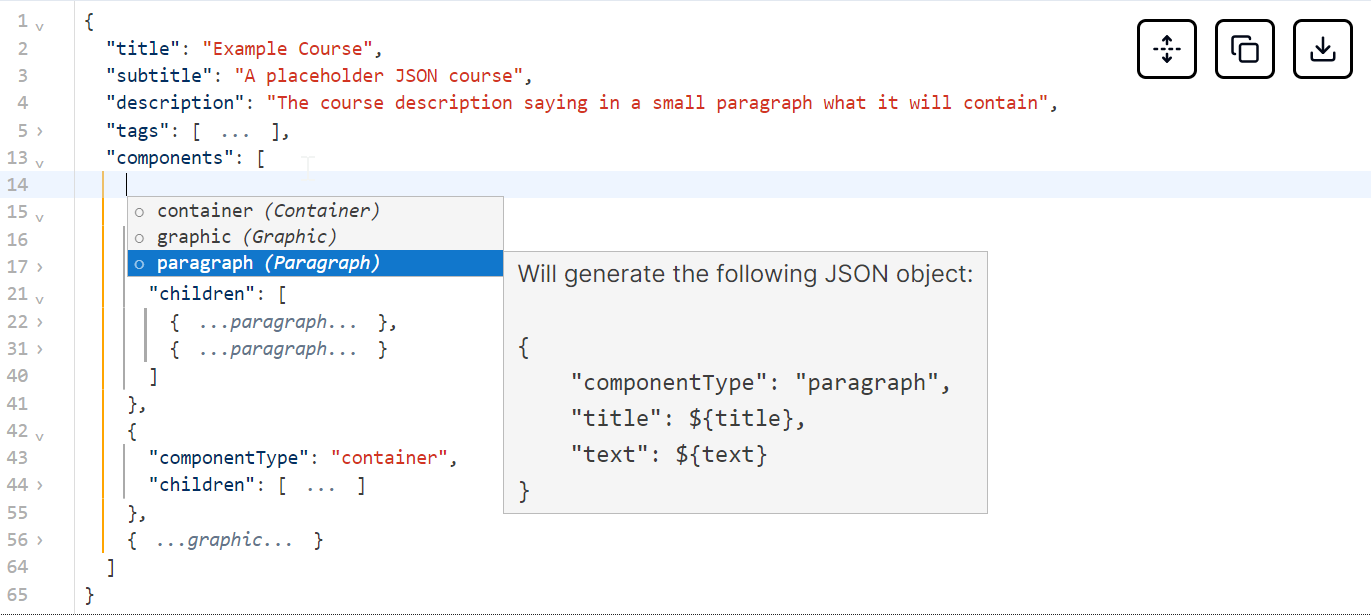
\includegraphics[scale=0.65]{images/json-editor-autocomplete-components.png}
    \caption{JSON Editor - Components Autocomplete Example}
    \label{fig:json-editor-autocomplete-components}
\end{figure}

\begin{figure}[hbt!]
    \centering
    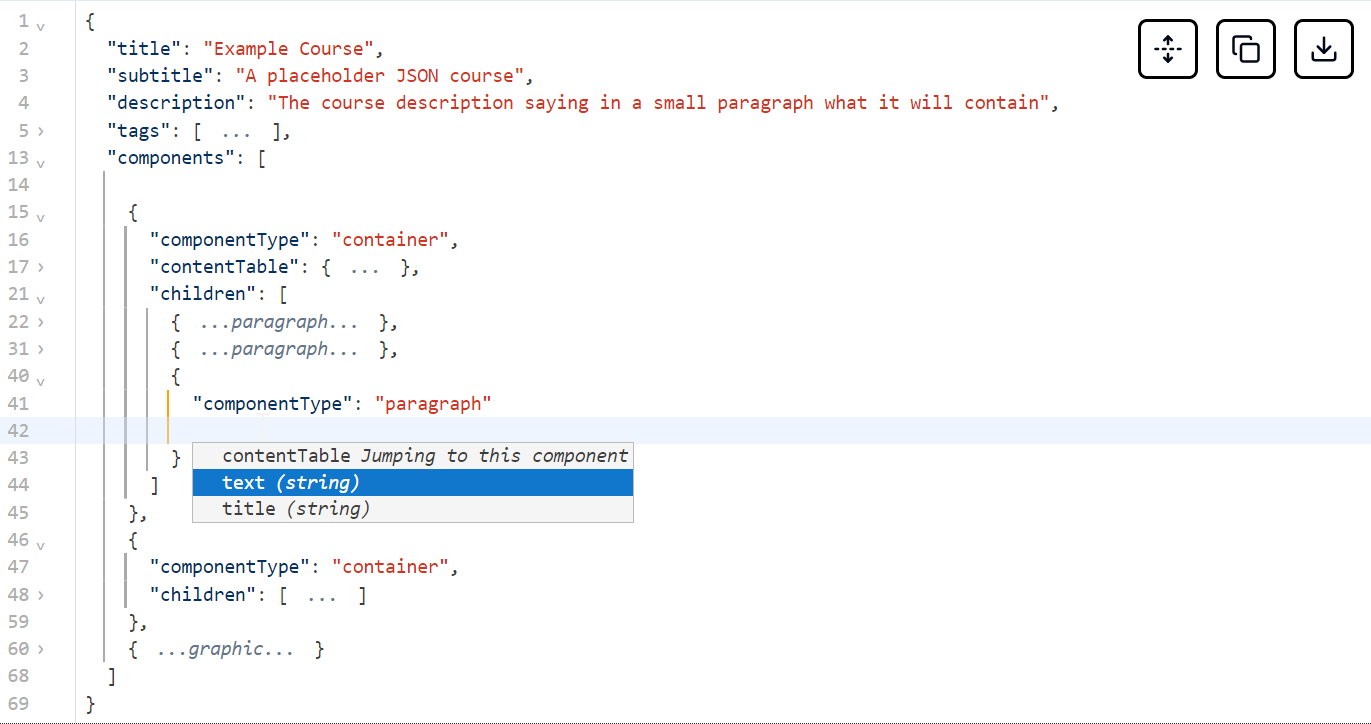
\includegraphics[scale=0.65]{images/json-editor-autocomplete-fields.png}
    \caption{JSON Editor - Properties Autocomplete Example}
    \label{fig:json-editor-autocomplete-fields}
\end{figure}

\noindent Autocomplete snippets can even get more dynamic, by providing code snippets that are always different when the suggestion is accepted. An example of this, is generating the \textbf{contentTable} property which will generate a unique UUID for each entry. The contentTable needs to have an unique id, as the table of contents has a \textbf{goto feature} that allows the user to navigate to the component that is clicked. The required UUIDs are generated by the \texttt{uuid} npm package, which is a simple and efficient way to generate unique identifiers.
\\\\
\noindent This is by far one of the most helpful features of the editor, as it can guide the user through the creation of a course, offering suggestions for components and parameters. The user can also learn about the components and their parameters by reading the suggestions. The autocomplete feature is also a good way to avoid typos, as the user can select the correct component or parameter from the list of suggestions.

\subsection{AutoRepair JSON}

\begin{figure}[h]
    \centering
    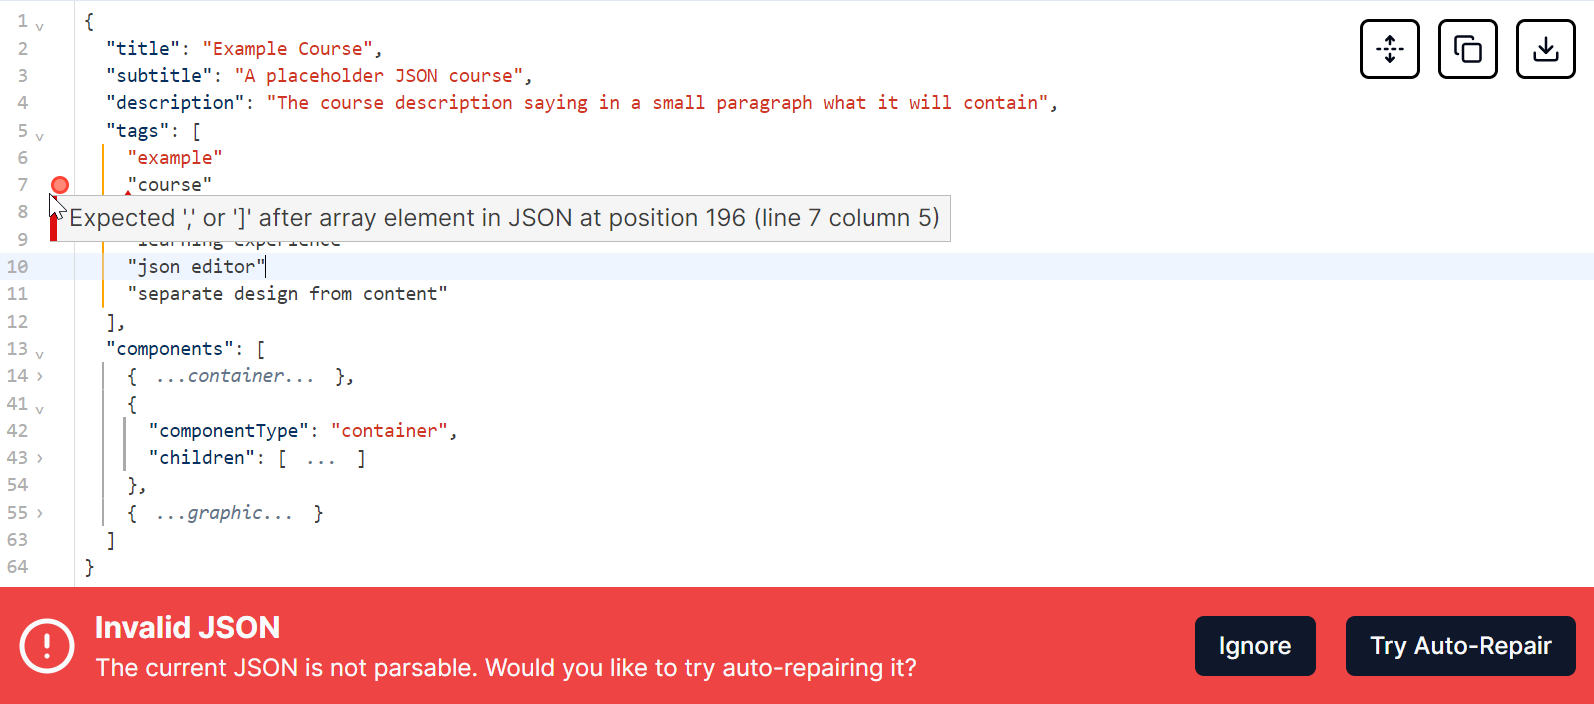
\includegraphics[scale=0.55]{images/json-editor-autorepair.png}
    \caption{JSON Editor - AutoRepair Prompt}
    \label{fig:json-editor-autorepair}
\end{figure}

\begin{figure}[h]
    \centering
    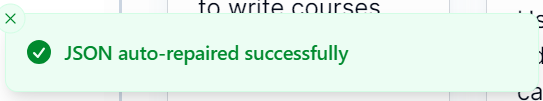
\includegraphics[scale=1]{images/json-editor-autorepair-success.png}
    \caption{JSON Editor - AutoRepair Success Toast}
    \label{fig:json-editor-autorepair-success}
\end{figure}

\begin{figure}[hbt!]
    \centering
    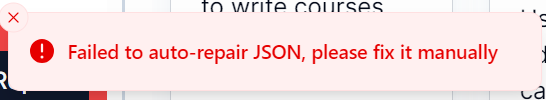
\includegraphics[scale=1]{images/json-editor-autorepair-error.png}
    \caption{JSON Editor - AutoRepair Error Toast}
    \label{fig:json-editor-autorepair-error}
\end{figure}

\noindent When working with JSONs you will often encounter the problem of missing commas, brackets, or quotes. This can be very frustrating, as the JSON will not be valid and the editor will not be able to parse it. To avoid this, the editor is equipped with an \textbf{AutoRepair} feature. The feature is implemented inside the \textbf{json-auto-repair-lint.ts} file, located inside the \hl{@/modules/courses/utils} folder.
\\\\
\noindent Inside the JSON Editor, whenever a JSON parse exception is encountered, one that does not belong to the custom linter, in the bottom of the editor an alert box will be displayed, which gives the user two options (see Figure \ref{fig:json-editor-autorepair}). They can choose to ignore the error, which will make the box disappear until the error changes or is fixed, or they can choose trying to auto-repair it. A \textbf{toast} message with the result of the auto-repair operation will be displayed in the bottom right corner of the screen (see Figures \ref{fig:json-editor-autorepair-success} and \ref{fig:json-editor-autorepair-error}).
\\\\
\noindent For auto-repairing, the \textbf{jsonrepair} npm package is used. It provides a lot of features regarding the JSON, besides handling commas, brackets, and quotes. The package can also handle the removal of comments, trailing commas, and other JSON specific problems. It helps with compatibility, as it also replaces Python and MongoDB specific syntax with the standard JSON syntax.
\\\\
\noindent It is important to keep in mind that the auto-repair feature is not a replacement for the linter. The linter is used to provide personalized messages for the user, while the auto-repair feature is used to quickly fix the JSON so it can be parsed. The linter will still display errors if the JSON is not correctly written, even after the auto-repair operation. There might even be times when the auto-repair operation will not be able to fix the JSON, but the linter will still be able to provide a message for the user.
\\\\
\noindent Its important to check the place of the error after the JSON is auto-repaired, as the auto-repair might decide that instead of adding a quote and a missing comma, it will concatenate the two strings. This is a rare case, but it can happen, and the user should be aware of it. Even if it occurs, it will be obvious in the live preview that the component is not displayed correctly.

\subsection{Live Preview}

\noindent The live preview is a feature that allows the user to see the course as it would be displayed on the web platform. The live preview is displayed in the right side of the editor (see Figure \ref{fig:live-preview-editor}), and it is updated in real-time as the user types.
\\\\
\noindent To make this possible, since usually the two sides (middle and right) are handled separately, a \textbf{React Context} is used to share the JSON content between them. A provider is created inside the \textbf{course-json-provider.tsx} file, located inside the \hl{@/modules/courses/context} folder. The provider is wrapped around the layout of the whole courses section. Of course, the provider should not be used outside the editor, although it is available everywhere in this section. For this reason, the course JSON from inside the provider is cleared when the route changes, using an \textbf{useEffect} that relies on Next.js' \textbf{usePath} hook.

\begin{figure}[h]
    \centering
    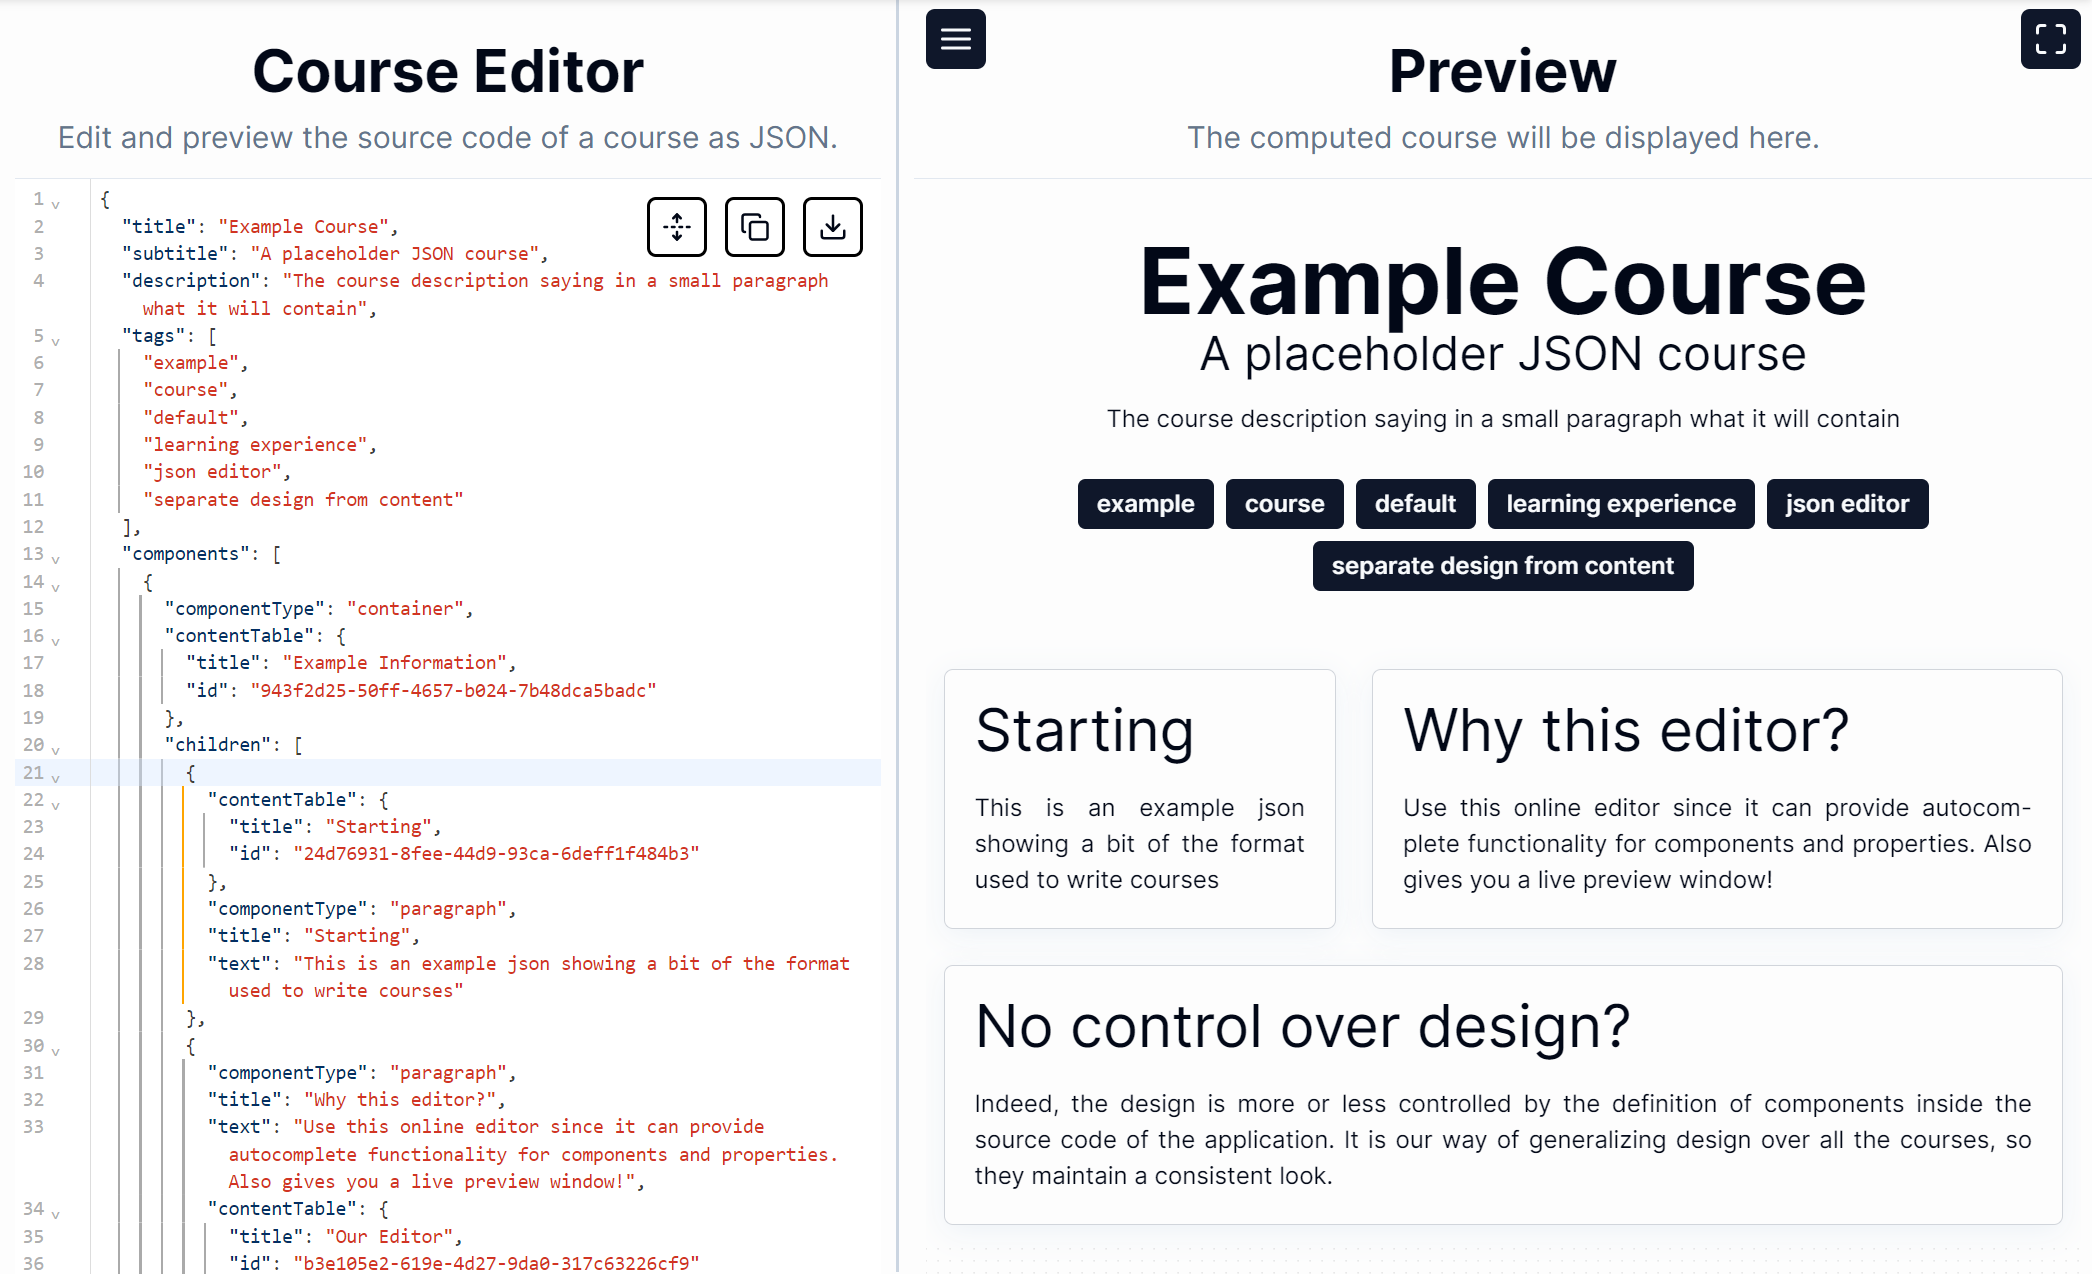
\includegraphics[scale=0.45]{images/live-preview-editor.png}
    \caption{JSON Editor with Live Preview}
    \label{fig:live-preview-editor}
\end{figure}
\newpage
\noindent To facilitate the \textbf{Save changes} option of the editor, the JSON is stored in two variables, initialCourseJSON and inEditCourseJSON. The two JSONs are used to compare the changes made by the user. If the user decides to save the changes, the inEditCourseJSON will be sent to the backend.
\\\\
\noindent To avoid desynchronization, the initialCourseJSON and the inEditCourseJSON need to be updated at the same time, when fetched from the database. For this reason they are both wrapped in the same variable, wholeJSON. To wholeJSON is exposed as courseJSON to the editor, along with three functions, setInitialCourseJSON and setInEditCourseJSON, that are used to update the JSONs, and internally use the setWholeJSON function to update the wholeJSON variable.
\\\\
\noindent Monitoring the inEditCourseJSON, the right side will rerender the live preview whenever the JSON changes. The live preview uses the actual course component, which was designed to allow for dynamic changes, by including error boundaries and having cached components based on the provided JSON.
\\\\
\noindent Since the right side might not be enough to fully visualize the course, in the top right corner a button is added that allows for a bigger display, by opening a dialog that spans over the entire page. Besides that, in the top left corner, a button for previewing the table of contents is added. The table of contents is a list of all the components that are present in the course, and it allows the user to navigate to a specific component by clicking on it. The user might not want to display all components inside the table, so only components annotated with the \textbf{contentTable} property are displayed. Based on their depth level, the components are indented, and the user can easily see the hierarchy of the course.

\section{Graphics/Diagrams}

Information can sometimes be better conveyed through graphics. For this reason, the web platform offers a graphic editor that can be used to create diagrams. Unlike the course editor, this one is not a code editor, but a visual editor (see Figure \ref{fig:graphic-editor}). The graphic editor is used to create graphics that can be used inside the course editor.

\begin{figure}[h]
    \centering
    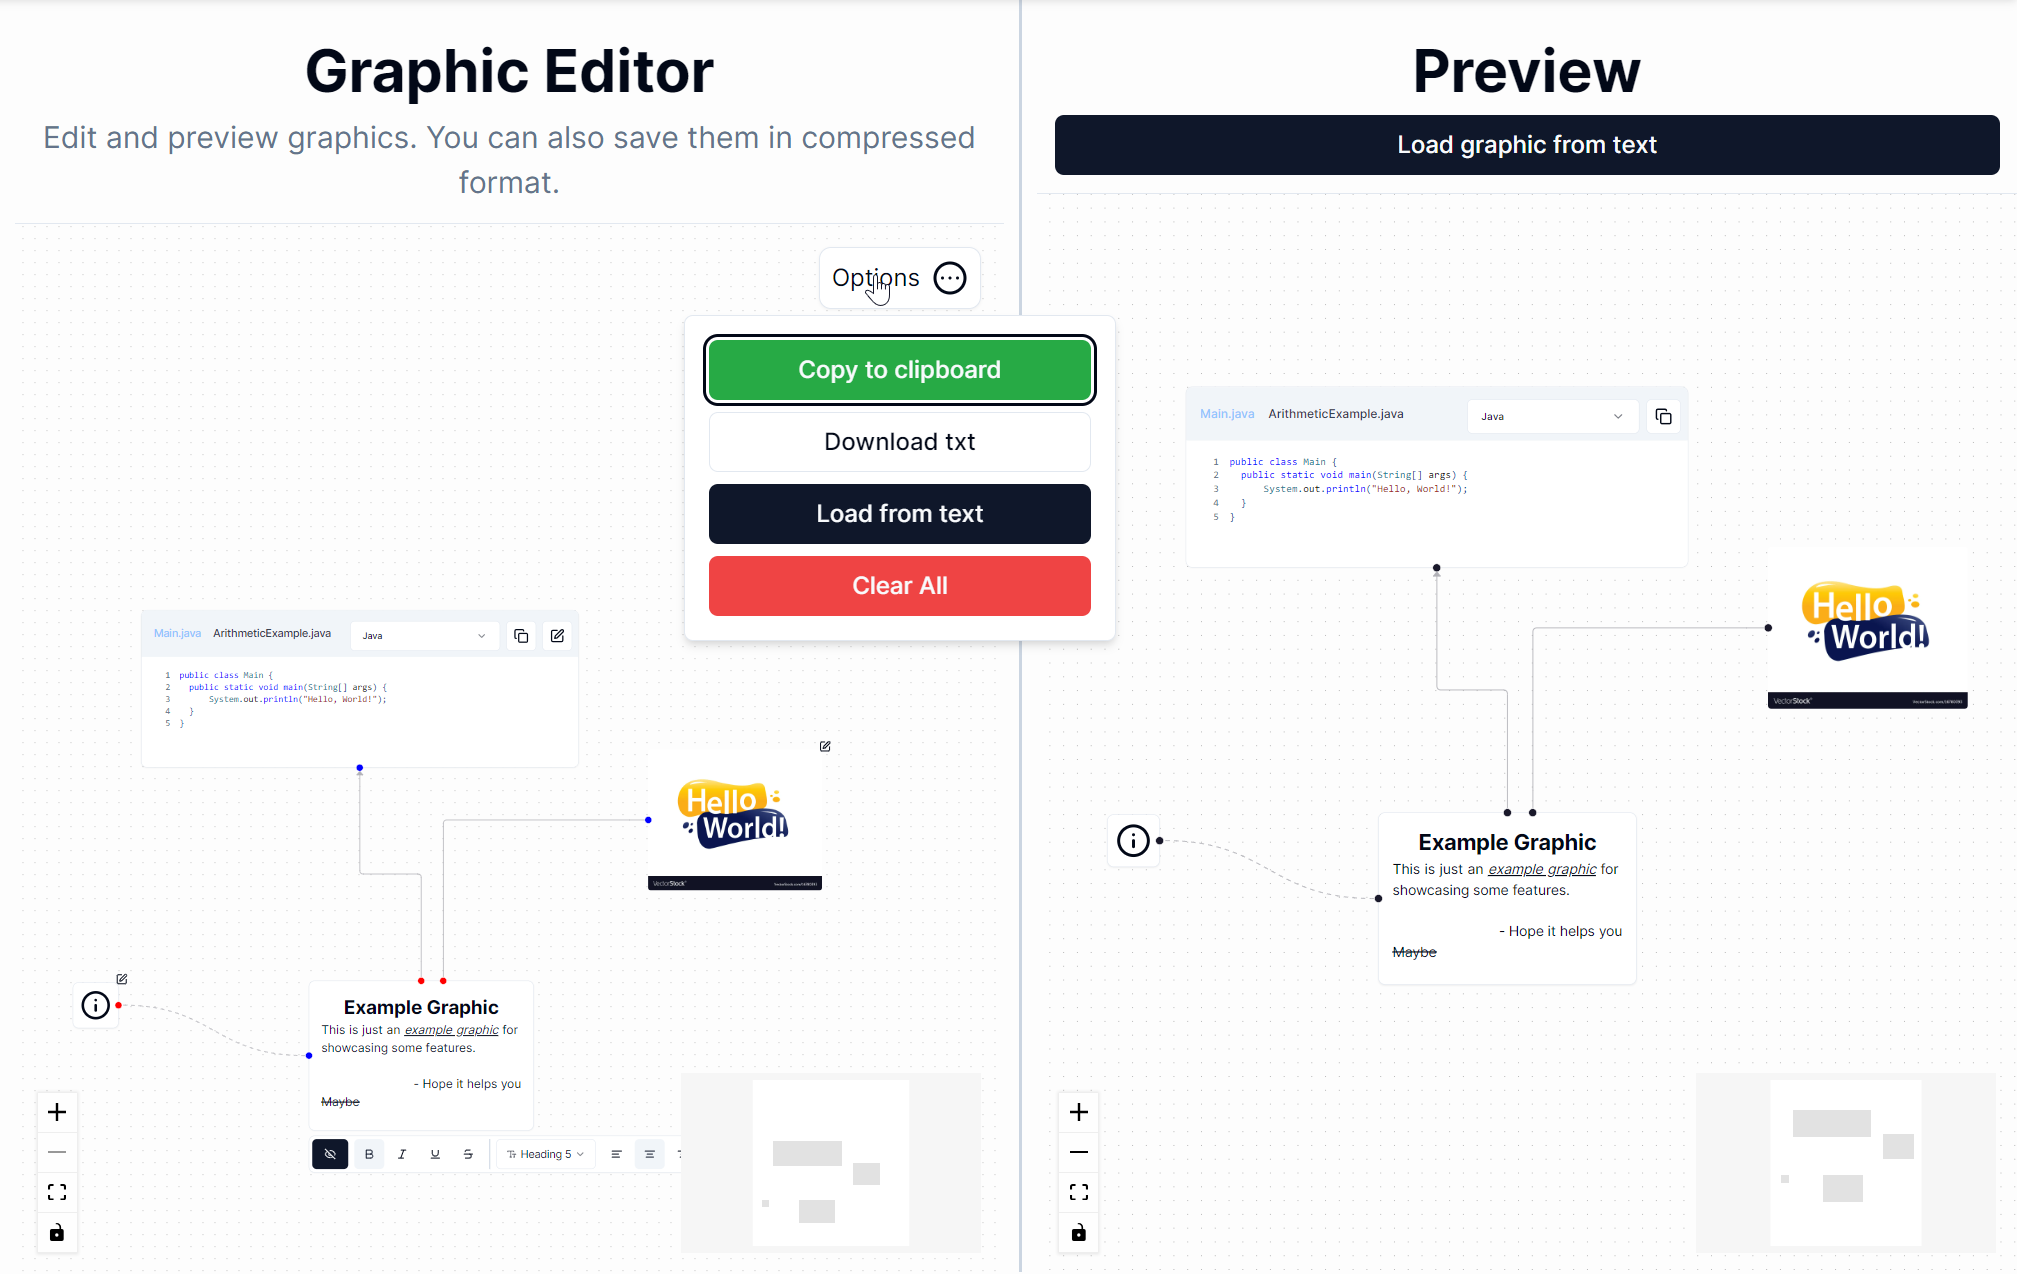
\includegraphics[scale=0.45]{images/graphic-editor.png}
    \caption{Graphic editor with example graphic}
    \label{fig:graphic-editor}
\end{figure}

\subsection{Diagrams Library}

\noindent For the graphics, the \textbf{ReactFlow} library \cite{reactflow} was chosen. This library offers a component with a graph like structure, that can be used to create diagrams. The library is very flexible, and it can be used to create a wide variety of diagrams, from flowcharts to mind maps.
\\\\\newpage
\noindent Elements are added to the graph via nodes and edges. Both the nodes and the edges offer various customization options, ReactFlow allowing developers to even create their own components for them. Besides that, the canvas itself is very customizable, allowing for zooming, panning, and even the creation of custom background elements. It also allows for the personalization of the actions menu.
\\\\
\noindent Besides the design customization, ReactFlow also offers dynamic interaction with the elements from the graph. The elements can be dragged, resized and connected. The canvas itself can be dynamically resized without causing elements inconsistencies.
\\\\
\noindent The state of the graph can also be stored in an external JSON, which can be used to recreate the graph at a later time. This is very useful for the web platform, as the graphics created by the user can be stored in the course JSON, and displayed in the course view. The JSON can also be used to recreate the graphic in the graphic editor, in case the user wants to make changes to it.
\\\\
\noindent The learning curve of this library also proved to be very low, as the documentation is very well written and the examples are very helpful.

\subsection{Nodes}

\noindent At the time at which this thesis was written, there are four types of nodes: image, code, rich text and information. More nodes might be added in the future, but the current ones are enough to cover a wide range of use cases. Besides the type of nodes, there exists two copies of each node, one for the graphic editor and one for the display inside the course. The nodes are stored in the \hl{@/modules/courses/components/graphic/nodes} folder.

\begin{figure}[h]
    \centering
    \begin{minipage}{0.45\textwidth}
        \centering
        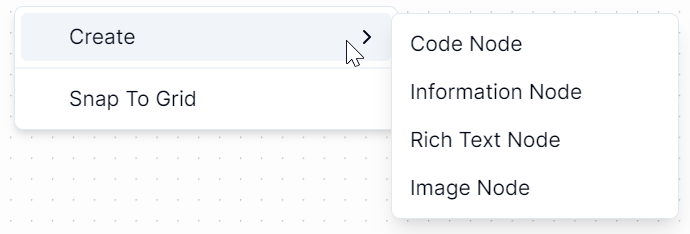
\includegraphics[width=1\linewidth]{images/canvas-context-menu.png}
    \end{minipage}%
    \hspace{0.1\textwidth}% 
    \begin{minipage}{0.45\textwidth}
        \centering
        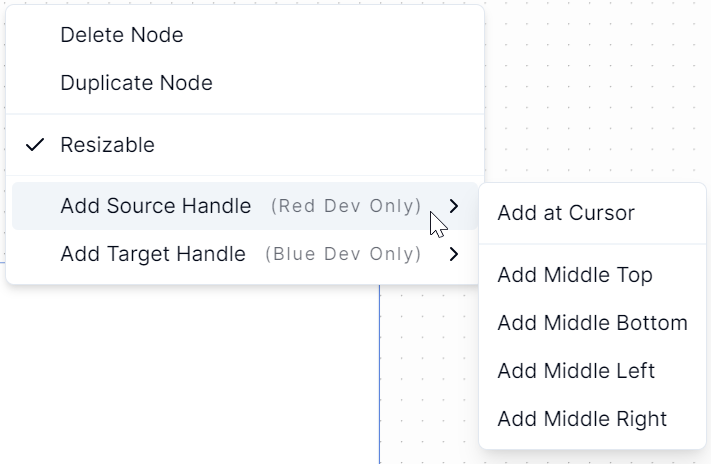
\includegraphics[width=1\linewidth]{images/node-context-menu.png}
    \end{minipage}
    \caption{Canvas and Node Context Menus}
    \label{fig:context-menus}
\end{figure}

\noindent For taking actions regarding nodes, the graphic editor relies on two context menus (Figure \ref{fig:context-menus}). The first one is the node context menu, which is displayed when right clicking on a node. The second one is the canvas context menu, which is displayed when right clicking on the canvas. The context menus are used to offer actions that can be taken on the nodes, such as creating a node at a given position, delete a selected one, or duplicate it. The context menus are stored in the \hl{@/modules/courses/components/graphic/context-menu} folder.
\\\\
\noindent The \textbf{rich text node} is a text editor itself, that gives you a bit more customization than just a textarea. For this, an equivalent for CodeMirror exists, named \textbf{ProseMirror}, which is a toolkit for building rich text WYSIWYG editors. To expand on the power of ProseMirror, a headless wrapper around it is used, to offer more out of the box extensions. The wrapper is \textbf{TipTap} \cite{tiptap}, that is also compatible with React. The editor is used to offer more customization options for the text, such as bold, italic, underline, lists, text alignment and so on. While very customizable, the functionalities of the editor are limited, as to focus on a consistent design, without too many overwhelming options.

\begin{figure}[hbt!]
    \centering
    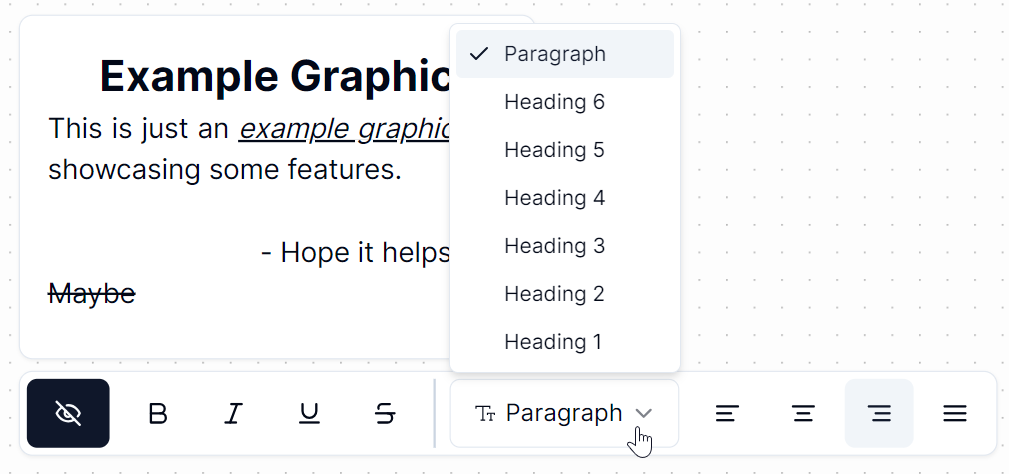
\includegraphics[scale=0.62]{images/rich-text-node.png}
    \caption{Rich text node with editor}
    \label{fig:rich-text-node}
\end{figure}

\noindent The \textbf{image node} is used to display images inside the graphic. Currently, images can only be added via a URL, but in the future, the user might be able to upload images from their computer. Since the node can be resized, an extra option is offered, to keep the aspect ratio of the image (see Figure \ref{fig:image-node-editor}).

\begin{figure}[hbt!]
    \centering
    \begin{minipage}{0.45\textwidth}
        \centering
        
\includegraphics[width=0.72\linewidth]{images/image-node.png}
        \caption{Initial Image Node}
        \label{fig:image-node}
    \end{minipage}%
    \hspace{0.1\textwidth}% 
    \begin{minipage}{0.45\textwidth}
        \centering
        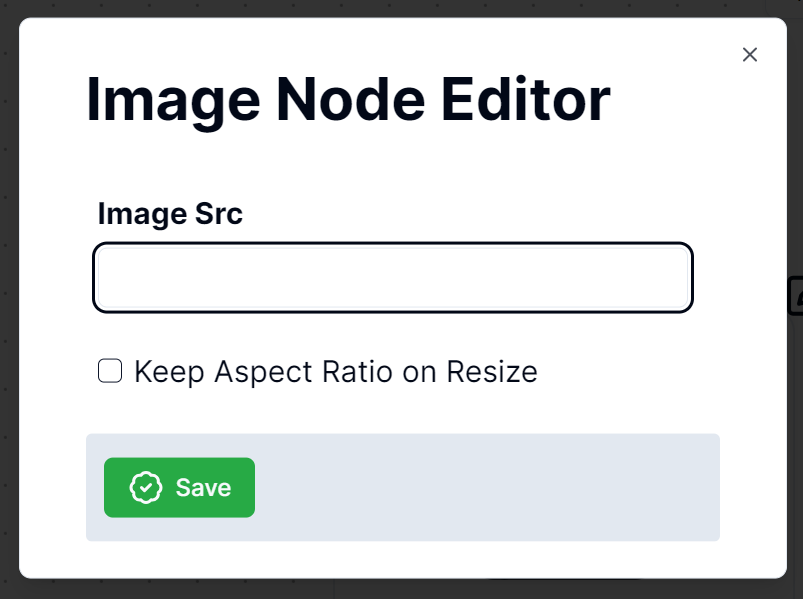
\includegraphics[width=1\linewidth]{images/image-node-editor.png}
        \caption{Image Node Editor}
        \label{fig:image-node-editor}
    \end{minipage}
\end{figure}

\noindent The \textbf{information node} is a small box with an information icon, that when hovered over, displays a tooltip with the information. This node is used to display information that is not directly visible in the graphic, as to not overwhelm the user. From its editor you can change the inner information and the side the tooltip should appear on.

\begin{figure}[hbt!]
    \centering
    \begin{minipage}{0.45\textwidth}
        \centering
        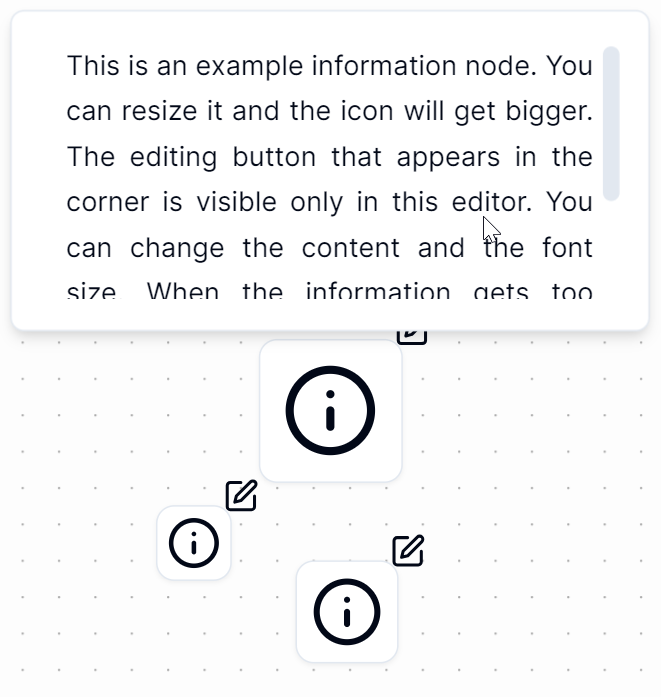
\includegraphics[width=1\linewidth]{images/information-node.png}
        \caption{Information Nodes}
        \label{fig:information-node}
    \end{minipage}%
    \hspace{0.1\textwidth}% 
    \begin{minipage}{0.45\textwidth}
        \centering
        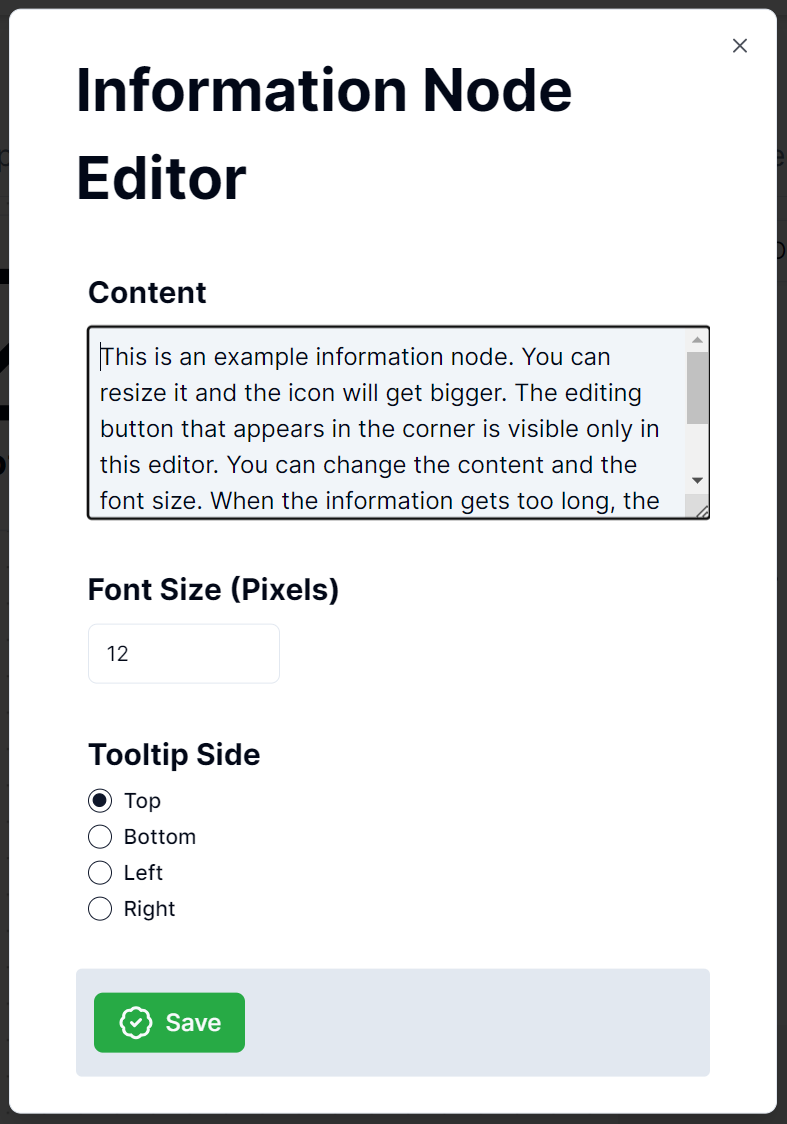
\includegraphics[width=1\linewidth]{images/information-node-editor.png}
        \caption{Information Node Editor}
        \label{fig:information-node-editor}
    \end{minipage}
\end{figure}
\noindent \\
\noindent The \textbf{code box node} is used to display code inside the graphic. For the highlight of the code, Prism.js \cite{prismjs} is used, which is a lightweight, extensible syntax highlighter. Prism.js is implemented in the web platform through a React wrapper, provided by the \textbf{prism-react-renderer} npm package. The code box node is used to display code snippets that are relevant to the graphic. The code box is designed to allow for multiple code snippets inside the display, either by having multiple files inside the code box, or by having a dropdown button that lets you change the language of the code snippet. Besides that, the code box contains a copy button, that will copy to clipboard the code from the active file. The editor of the code box is also very complex, and it relies on a JSON editor is as well. To avoid having a very long JSON, for the actual code snippets placeholders are used. You can create multiple snippets inside the editor, and then reference them inside the JSON configuration. The configuration itself is for specifying the languages the code box supports and the files that should be displayed.

\begin{figure}[hbt!]
    \centering
    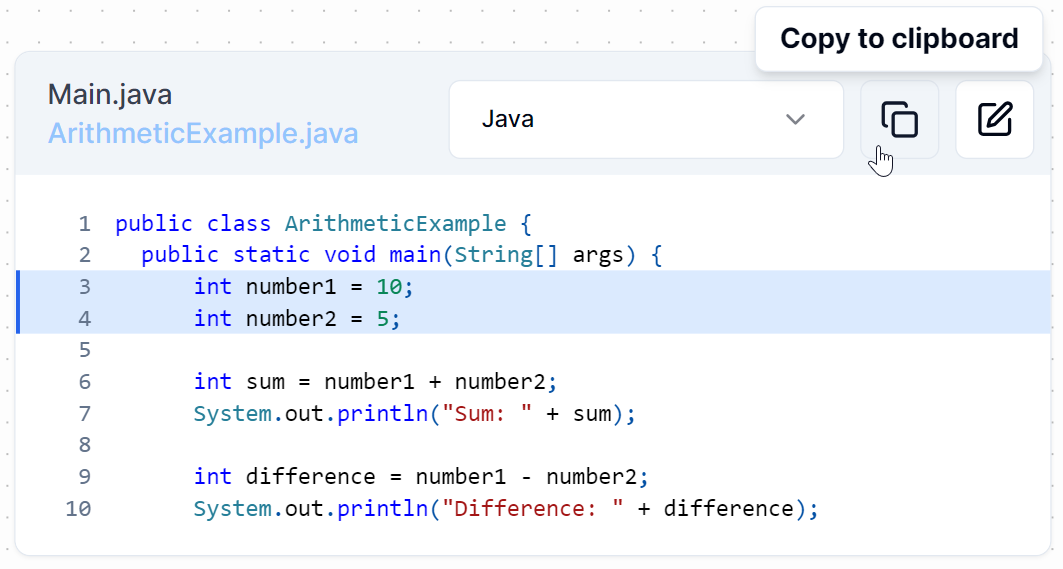
\includegraphics[scale=0.65]{images/code-node.png}
    \caption{Code node with example code}
    \label{fig:code-node}
\end{figure}
\newpage
\noindent If in the future there will be a need for more nodes, the graphic editor can be extended without affecting the current ones. If some of the current nodes will change or be deleted, the graphic's JSON like structure allows for simply ignoring the nodes that are not recognized.

\subsection{Edges}

\noindent By edges, it should be understood the lines between the nodes. The edges are used to show a connection between two nodes. They also have different customization options, from their display to the handles of the node they are connected with. The edges are stored in the \hl{@/modules/courses/components/graphic/edges} folder.
\\\\
\noindent The edges also have a context menu, that is displayed when right-clicking on an edge (see Figure \ref{fig:edges-context-menu}). The context menu is used to offer actions that can be taken on the edges, such as changing the line style, if it should be dashed or not, if it should have a marker at the start/end. The context menu is stored in the \hl{@/modules/courses/components/graphic/context-menu} folder.
\\\\
\noindent Edges can be straight, bezier, step or smoothstep (see Figure \ref{fig:edges}). The \textbf{straight edge} is the most basic one, connecting two nodes with a straight line. The \textbf{bezier edge} is a curved line, that connects two nodes. The \textbf{step edge} is a line that connects two nodes with a series of horizontal and vertical lines. The \textbf{smoothstep edge} is a line that connects two nodes with multiple straight lines, that are smoothed out at the corners. The markers that can be placed at the start and the end of the edges can be open/closed arrows or circles. They are optional, and can be added or removed from the context menu. When an edge becomes dashed, it will also have a flowing animation, from start to end.

\begin{figure}[hbt!]
    \centering
    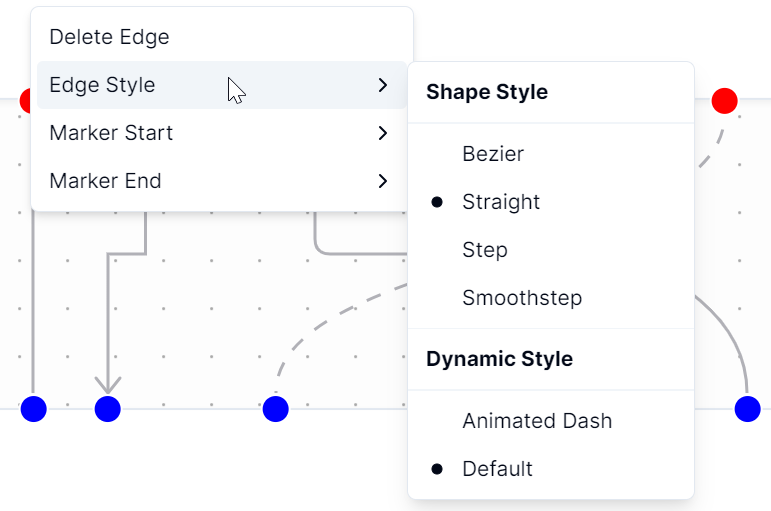
\includegraphics[scale=0.75]{images/edges-context-menu.png}
    \caption{Edge context menu}
    \label{fig:edges-context-menu}
\end{figure}

\begin{figure}[hbt!]
    \centering
    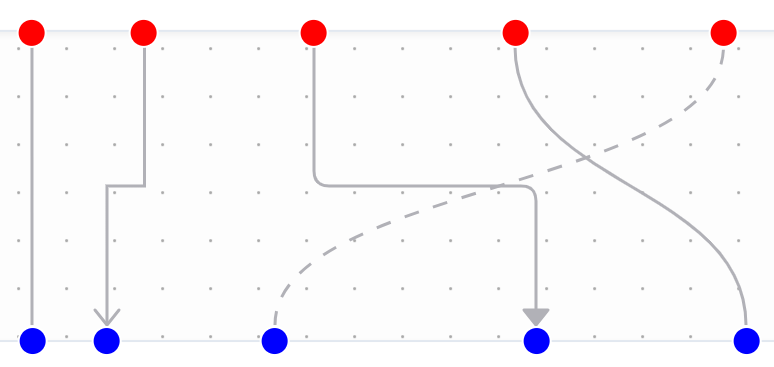
\includegraphics[scale=0.75]{images/edges.png}
    \caption{Edge types}
    \label{fig:edges}
\end{figure}

\noindent More customization can be added to the edges in the future, such as custom colors, thickness, or even animations. The current customization options are enough to cover a wide range of use cases, and they are very easy to use.
\\\\
\noindent The edges are connected to a node at specific points called handlers. The customization of these handles allows for easier understanding of the connections, as they can be added in dynamic positions of the node, while with fixed positions you might end up with overlapping lines. You can still add them in cardinal positions, middle right, middle left, middle top, middle button, but they can also be added relative to the position of the cursor.

\subsection{Graphic Object}

\noindent To avoid having to store graphics as JSON entities in the database, and giving them a tighter integration inside the course JSON a solution had to be found to make the graphic object a much more compact entity.
\\\\
\noindent To achieve this, the first thought was to store the graphic as a base64 string. This would have been a good solution, as the graphic would be stored as a string, and it would be easy to display it inside the course view. The problem with this solution is that the graphic would be very long, and it would take a lot of space.
\\\\
\noindent Since a base64 string is more compact than the raw JSON stringified, this approach was kept, but the source it is applied on had to change. For this reason, a compression algorithm on the stringified JSON, or on the bytes of the JSON themselves, could be applied to improve the memory usage. The graphic structure could for sure benefit of compression, as the JSON structure is very repetitive, and the same properties are used multiple times.
\\\\
\noindent In the end, the \textbf{JSONCrush} library \cite{jsoncrush} was used. It compresses JSON similar to the \textbf{zip} algorithm. Comparing the base64 string of the stringified JSON to the crushed JSON that the library outputs, it can be seen that the crushed JSON is much shorter, especially for more complex graphics.
\\\\
\noindent The graphic object ends up being a portable base64 string, obtained by stringifying the JSON, crushing it with the library, and finally converting it. When displaying the graphic, either in the editor or the course component, the process is reversed and the obtained JSON is processed by ReactFlow.

\section{Security}

Inside a web platform, we can't rely on the user to always have good intentions, so security for private data can't be implemented inside the frontend. For this reason, any private logic as session handling or database access is done either directly in the Spring Boot backend, or through the backend of the NextJS, the middleware. The frontend is only responsible for the visual representation of the data, and the user interaction with it.

\subsection{NextAuth Configuration}

\noindent The web platform uses \textbf{NextAuth} \cite{nextauth} for authentication. I opted for an open source solution that is well maintained and has a lot of features. NextAuth is a complete authentication solution for Next.js applications. It is easy to use, and it offers a lot of providers, such as Google, Facebook, Twitter, GitHub, and many more.
\newpage
\noindent In this web platform, three files are used for setting up NextAuth. The \textbf{route.ts} file, located inside the \hl{@/app/(users)/api/auth/[...nextauth]} folder, is used to catch all routes handled by nextauth. The \textbf{auth.config.ts} file which is responsible for configuration of the providers and adding callbacks, that is located inside the \hl{@/modules/users/next\_auth} folder. The \textbf{nextauth.d.ts} file, located at the root of the frontend project, is used to declare the types of the session object.
\\\\
\noindent The \textbf{route.tsx} is the entry point for NextAuth. It uses the configuration options defined in \textbf{auth.config.ts} to create a handler, that is exported using the GET and POST methods. Inside the \textbf{auth.config.ts} file, various options for NextAuth are declared. Firstly, the default login, logout and error pages are overridden with custom implemented routes. The \textbf{providers} array is used to declare the oauth2 sources that are used for authentication. The \textbf{callbacks} object is used to declare the callbacks that are used for the authentication process. The signIn, jwt and session callbacks are added here, to help process the user data. The \textbf{events} object is used to declare a signOut event, that will also signal the action to the backend.
\\\\
\noindent The \textbf{nextauth.d.ts} file is used to extend the types of the session and token objects. A user interface is declared that adds authorities and backend tokens to use inside the session object. The jwt object also receives this user.
\\\\
\noindent Although not a file with the express purpose of handling NextAuth, the \textbf{middleware.ts} file also uses a middleware object provided by NextAuth. The \textbf{withAuth} middleware is used to protect routes that require authentication. The middleware is used to check if the user is authenticated, and if not, redirect them to the login page.
\\\\
\noindent \textbf{Attention!} It is important to note that the Next's middleware can only intercept requests made between the client and the backend of the NextJS project! If requests to the Spring Boot backend are made directly inside the client, the middleware will not be able to intercept them.

\subsection{OAuth2}

\noindent To avoid the storage of passwords, the web platform uses OAuth2 for authentication. The connection to the third party providers is done through the NextAuth library. The user can choose to authenticate with Discord and GitHub. To connect to these providers, OAuth2 applications have been set up on the respective platforms. The client ID and client secret are stored in the environment variables of the NextJS backend.
\\\\
The access token obtained from the provider is used to further authenticate the user with the Spring Boot authorization server. The access token is sent to the backend, where it is validated and used to create a JWT token. The JWT token is then sent back to the frontend, and stored inside the session object. Two tokens are used, an access token that gives the user access to the resources, and a refresh token that is used to obtain a new access token when the old one expires.
\\\\
\noindent The custom login page, which contains the login card displayed in Figure \ref{fig:login-card}, uses the \textbf{signIn} method provided by NextAuth to initiate the OAuth2 flow with the specified provider. The method accepts two parameters, the name of the provider and the options. Only a callbackUrl is provided as an option, to redirect the user back to the login page after the authentication process is done. The \textbf{signIn} method is called when the user clicks on the login button of the provider.
\\\\
\noindent In the future, more providers can be added, such as Google, Facebook, Twitter, or even custom providers. The process is simple, as the NextAuth library offers a lot of providers, and the setup is easy.

\begin{figure}[hbt!]
    \centering
    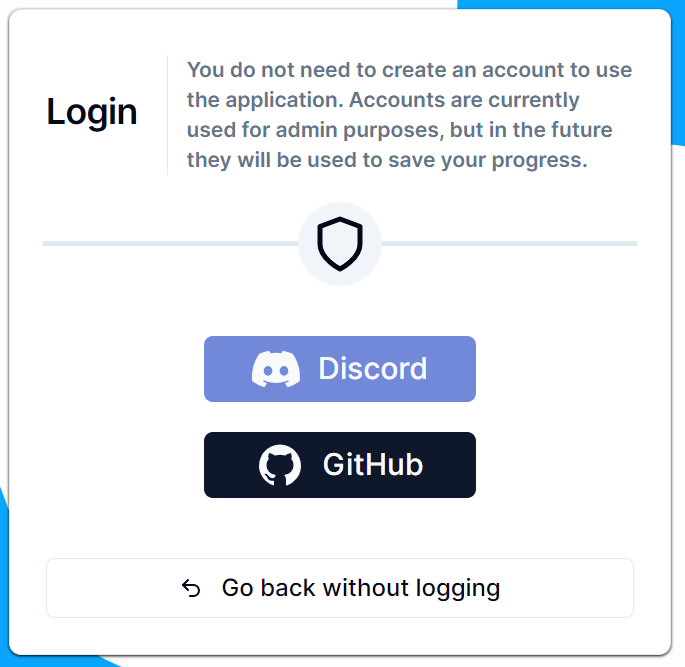
\includegraphics[scale=0.9]{images/login-card.png}
    \caption{Custom Login Card}
    \label{fig:login-card}
\end{figure}


\subsection{User Sessions}

\noindent The user session is stored inside the session object, which is provided by NextAuth. By default, the session object provides data such as email, username and so on. In the modified version used in this web platform, the session holds the user id, their authorities and access and refresh tokens that are used to authenticate the user with the backend.
\\\\
\noindent A global provider, \textbf{SessionEnsure} is used to monitor the session, forcefully signing out the user if the Spring Boot backend session is invalidated. In the context of JWTs, that would mean when the refresh token expires or is marked as invalid. To refresh the access token, two mechanics are employed. Firstly, the jwt callback in NextAuth's configuration is used to refresh the access token whenever it expires. Secondly, in the \textbf{SWR config}, a fetcher that handles onError events is used to refresh the access token whenever a 401 error is encountered.